\documentclass[11pt,]{article}
\usepackage[left=1in,top=1in,right=1in,bottom=1in]{geometry}
\newcommand*{\authorfont}{\fontfamily{phv}\selectfont}
\usepackage[]{mathpazo}


  \usepackage[T1]{fontenc}
  \usepackage[utf8]{inputenc}



\usepackage{abstract}
\renewcommand{\abstractname}{}    % clear the title
\renewcommand{\absnamepos}{empty} % originally center

\renewenvironment{abstract}
 {{%
    \setlength{\leftmargin}{0mm}
    \setlength{\rightmargin}{\leftmargin}%
  }%
  \relax}
 {\endlist}

\makeatletter
\def\@maketitle{%
  \newpage
%  \null
%  \vskip 2em%
%  \begin{center}%
  \let \footnote \thanks
    {\fontsize{18}{20}\selectfont\raggedright  \setlength{\parindent}{0pt} \@title \par}%
}
%\fi
\makeatother




\setcounter{secnumdepth}{3}

\usepackage{color}
\usepackage{fancyvrb}
\newcommand{\VerbBar}{|}
\newcommand{\VERB}{\Verb[commandchars=\\\{\}]}
\DefineVerbatimEnvironment{Highlighting}{Verbatim}{commandchars=\\\{\}}
% Add ',fontsize=\small' for more characters per line
\usepackage{framed}
\definecolor{shadecolor}{RGB}{248,248,248}
\newenvironment{Shaded}{\begin{snugshade}}{\end{snugshade}}
\newcommand{\KeywordTok}[1]{\textcolor[rgb]{0.13,0.29,0.53}{\textbf{#1}}}
\newcommand{\DataTypeTok}[1]{\textcolor[rgb]{0.13,0.29,0.53}{#1}}
\newcommand{\DecValTok}[1]{\textcolor[rgb]{0.00,0.00,0.81}{#1}}
\newcommand{\BaseNTok}[1]{\textcolor[rgb]{0.00,0.00,0.81}{#1}}
\newcommand{\FloatTok}[1]{\textcolor[rgb]{0.00,0.00,0.81}{#1}}
\newcommand{\ConstantTok}[1]{\textcolor[rgb]{0.00,0.00,0.00}{#1}}
\newcommand{\CharTok}[1]{\textcolor[rgb]{0.31,0.60,0.02}{#1}}
\newcommand{\SpecialCharTok}[1]{\textcolor[rgb]{0.00,0.00,0.00}{#1}}
\newcommand{\StringTok}[1]{\textcolor[rgb]{0.31,0.60,0.02}{#1}}
\newcommand{\VerbatimStringTok}[1]{\textcolor[rgb]{0.31,0.60,0.02}{#1}}
\newcommand{\SpecialStringTok}[1]{\textcolor[rgb]{0.31,0.60,0.02}{#1}}
\newcommand{\ImportTok}[1]{#1}
\newcommand{\CommentTok}[1]{\textcolor[rgb]{0.56,0.35,0.01}{\textit{#1}}}
\newcommand{\DocumentationTok}[1]{\textcolor[rgb]{0.56,0.35,0.01}{\textbf{\textit{#1}}}}
\newcommand{\AnnotationTok}[1]{\textcolor[rgb]{0.56,0.35,0.01}{\textbf{\textit{#1}}}}
\newcommand{\CommentVarTok}[1]{\textcolor[rgb]{0.56,0.35,0.01}{\textbf{\textit{#1}}}}
\newcommand{\OtherTok}[1]{\textcolor[rgb]{0.56,0.35,0.01}{#1}}
\newcommand{\FunctionTok}[1]{\textcolor[rgb]{0.00,0.00,0.00}{#1}}
\newcommand{\VariableTok}[1]{\textcolor[rgb]{0.00,0.00,0.00}{#1}}
\newcommand{\ControlFlowTok}[1]{\textcolor[rgb]{0.13,0.29,0.53}{\textbf{#1}}}
\newcommand{\OperatorTok}[1]{\textcolor[rgb]{0.81,0.36,0.00}{\textbf{#1}}}
\newcommand{\BuiltInTok}[1]{#1}
\newcommand{\ExtensionTok}[1]{#1}
\newcommand{\PreprocessorTok}[1]{\textcolor[rgb]{0.56,0.35,0.01}{\textit{#1}}}
\newcommand{\AttributeTok}[1]{\textcolor[rgb]{0.77,0.63,0.00}{#1}}
\newcommand{\RegionMarkerTok}[1]{#1}
\newcommand{\InformationTok}[1]{\textcolor[rgb]{0.56,0.35,0.01}{\textbf{\textit{#1}}}}
\newcommand{\WarningTok}[1]{\textcolor[rgb]{0.56,0.35,0.01}{\textbf{\textit{#1}}}}
\newcommand{\AlertTok}[1]{\textcolor[rgb]{0.94,0.16,0.16}{#1}}
\newcommand{\ErrorTok}[1]{\textcolor[rgb]{0.64,0.00,0.00}{\textbf{#1}}}
\newcommand{\NormalTok}[1]{#1}

\usepackage{graphicx,grffile}
\makeatletter
\def\maxwidth{\ifdim\Gin@nat@width>\linewidth\linewidth\else\Gin@nat@width\fi}
\def\maxheight{\ifdim\Gin@nat@height>\textheight\textheight\else\Gin@nat@height\fi}
\makeatother
% Scale images if necessary, so that they will not overflow the page
% margins by default, and it is still possible to overwrite the defaults
% using explicit options in \includegraphics[width, height, ...]{}
\setkeys{Gin}{width=\maxwidth,height=\maxheight,keepaspectratio}

\title{Cambio en la línea de costa en la playa Najayo  }



\author{\Large Carolain Pérez Ureña\vspace{0.05in} \newline\normalsize\emph{Estudiante, Universidad Autónoma de Santo Domingo (UASD)}  }


\date{}

\usepackage{titlesec}

\titleformat*{\section}{\normalsize\bfseries}
\titleformat*{\subsection}{\normalsize\itshape}
\titleformat*{\subsubsection}{\normalsize\itshape}
\titleformat*{\paragraph}{\normalsize\itshape}
\titleformat*{\subparagraph}{\normalsize\itshape}

\titlespacing{\section}
{0pt}{36pt}{0pt}
\titlespacing{\subsection}
{0pt}{36pt}{0pt}
\titlespacing{\subsubsection}
{0pt}{36pt}{0pt}





\newtheorem{hypothesis}{Hypothesis}
\usepackage{setspace}

\makeatletter
\@ifpackageloaded{hyperref}{}{%
\ifxetex
  \PassOptionsToPackage{hyphens}{url}\usepackage[setpagesize=false, % page size defined by xetex
              unicode=false, % unicode breaks when used with xetex
              xetex]{hyperref}
\else
  \PassOptionsToPackage{hyphens}{url}\usepackage[unicode=true]{hyperref}
\fi
}

\@ifpackageloaded{color}{
    \PassOptionsToPackage{usenames,dvipsnames}{color}
}{%
    \usepackage[usenames,dvipsnames]{color}
}
\makeatother
\hypersetup{breaklinks=true,
            bookmarks=true,
            pdfauthor={Carolain Pérez Ureña (Estudiante, Universidad Autónoma de Santo Domingo (UASD))},
             pdfkeywords = {línea de costa, playa pescadores, transectos, beachrock, imagenes
satelitales, imágenes aéreas, perfil de playa, clastos.},  
            pdftitle={Cambio en la línea de costa en la playa Najayo},
            colorlinks=true,
            citecolor=blue,
            urlcolor=blue,
            linkcolor=magenta,
            pdfborder={0 0 0}}
\urlstyle{same}  % don't use monospace font for urls

% set default figure placement to htbp
\makeatletter
\def\fps@figure{H}
\makeatother

\usepackage{float} \usepackage{pdflscape}
\newcommand{\blandscape}{\begin{landscape}}
\newcommand{\elandscape}{\end{landscape}}


% add tightlist ----------
\providecommand{\tightlist}{%
\setlength{\itemsep}{0pt}\setlength{\parskip}{0pt}}

\begin{document}
	
% \pagenumbering{arabic}% resets `page` counter to 1 
%
% \maketitle

{% \usefont{T1}{pnc}{m}{n}
\setlength{\parindent}{0pt}
\thispagestyle{plain}
{\fontsize{18}{20}\selectfont\raggedright 
\maketitle  % title \par  

}

{
   \vskip 13.5pt\relax \normalsize\fontsize{11}{12} 
\textbf{\authorfont Carolain Pérez Ureña} \hskip 15pt \emph{\small Estudiante, Universidad Autónoma de Santo Domingo (UASD)}   

}

}








\begin{abstract}

    \hbox{\vrule height .2pt width 39.14pc}

    \vskip 8.5pt % \small 

\noindent Se ha estudiado la transformación de la línea costera en playa Najayo
específicamente en la parte de los pescadores, San Cristóbal, sur de
República Dominicana. Se efectuaron diferentes métodos para una
evaluación más precisa de la vulnerabilidad y riesgo que tiene esta zona
litoral. Entre los cuales se usaron el estudio de imágenes satelitales
hechas entre los años 2013-2019, análisis granulométrico, delimitación
de la costa, generación de perfiles de playa, entre otras herramientas
digitales. Se ha evidenciado un cambio en la playa y un proceso de
retrogradación y progradación importante en estos últimos siete años, se
determinó que los fenómenos meteorológicos, la crecida del nivel del
mar, la dirección del viento, la circulación de las corrientes, y la
actividad humana son influyentes en dicho cambio.


\vskip 8.5pt \noindent \emph{Keywords}: línea de costa, playa pescadores, transectos, beachrock, imagenes
satelitales, imágenes aéreas, perfil de playa, clastos. \par

    \hbox{\vrule height .2pt width 39.14pc}



\end{abstract}


\vskip 6.5pt


\noindent  \section{Introducción}\label{introducciuxf3n}

La playa es la zona donde se depositan y se acumulan sedimentos
arrastrados principalmente por las olas. Estos sedimentos pueden ser
finos o gruesos. Es fundamental que la acumulación de material sea mayor
que la erosión en el litoral costero para la formación de una playa, así
como su área geomórfologica en conjunto.

La franja de tierra que tiene contacto e interacción con el medio
acuático es la costa. Por tanto, es en esta parte de la playa donde más
cambios se registran, tanto a escala geológica como histórica ancestral
y reciente. El origen de estas transformaciones son debidas
principalemnte por la oscilación de aguas marinas (Pedraza Gilsanz,
1996). Los efectos de estas alteraciones se traducen en un retroceso
acelerado de la costa, que se evidencia a través de registro de imágenes
aéreas, las cuales se analizan para dar seguimiento a los cambios
ocurridos en las costas(Ortiz Pérez, 1992).

La convergencia entre la zona marina y la terrestre produce unos
fenómenos que tienden a afectar las costas, conocidos como procesos
físicos litorales. Entre estos se distinguen los de tipo marítimo
(oleaje, corrientes, mareas) geológios (tsunamis), climáticos (vientos,
huracanes) y continentales (erosión hídrica y depósito de sedimentos
fluviales).

Los cambios más significativos en los últimos años son producidos por la
crecida del nivel del mar, así como por la presión de las olas que
provoca el desgaste y sedimentación en las costas. Esta acción
hidráulica provoca una modelación fisiográfica, que según Pedraza
Gilsanz (1996) puede dar lugar a distintos tipos de costas como por
ejemplo de ría, de fiordo, de cala, de isla barrera, arenosas o playas
estabilizadas, de delta, entre otras. Por otra parte, según su dinámica,
las costas se clasifican en de progradación, estacionaria y de
retrogradación (Codignotto, 1997).

En determinadas condiciones se acumula \emph{beachrock} o roca de playa,
la cual es una roca sedimentaria friable bien cementada que consiste en
una mezcla variable de sedimento de grava, arena y limo cementada con
minerales de carbonato. El carbonato de calcio se encarga de fosilizar
el \emph{beachrock}, dando lugar a playas rocosas. Dependiendo de la
ubicación, el sedimento puede consistir en una mezcla variable de
conchas, fragmentos de coral, fragmentos de roca de diferentes tipos y
otros materiales (Jackson, 2005). En las costas en retirada, los
afloramientos de roca de playa pueden ser evidentes en alta mar donde
actúan como una barrera contra la erosión costera. La presencia de roca
de playa también puede inducir deficiencia de sedimento en una playa y
sincronizar su régimen de olas.

El litoral sur de República Dominicana contiene playas idóneas para el
estudio de los fenómenos y tipos de depósitos mencionados. Un caso
típico es la playa Najayo, la cual es una pequeña ensenada labrada en
forma de ``muesca'' dentro del sistema de terrazas arrecifales
plio-cuaternarias del litoral sur dominicano, en la provincia San
Cristóbal, región administrativa de Valdesia. Litológicamente, la playa
y su entorno están compuestos de arena y gravas bioclásticas formando el
cordón litoral, en el fondo de valle conglomerado, gravas, arenas,
caliza arrecifal, calciruditas y calcarenitas (Mollat, Wagner, Cepek, \&
Weiss, 2004) (ver figura \ref{mapa_geologico}).

\begin{figure}
\centering
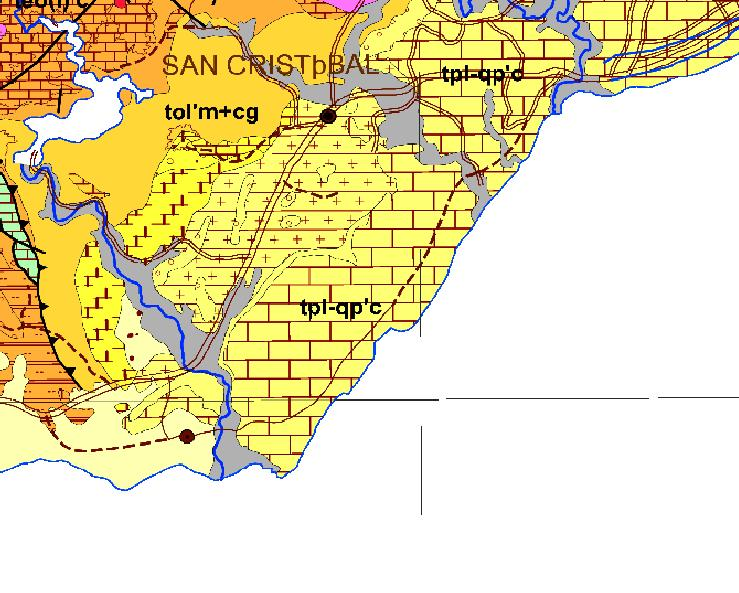
\includegraphics[height=3.64583in]{mapa geologico de najayo.jpg}
\caption{Mapa Geológico de República Dominicana, escala 1:250,000
\label{mapa_geologico}}
\end{figure}

La playa de Najayo limita al norte con una costa acantilada, y se
extiende al sudoeste siguiendo un trazado relativamente recto, con
algunas interrupciones donde afloran rocas del sustrato y depósitos de
playa tipo beachrock. Convencionalmente, se divide en dos sectores: 1)
Playa de los Pescadores, que ocupa los dos tercios septentrionales del
área, donde también desemboca el arroyo Rolón, y donde se localizan
algunos afloramientos de beachrock; 2) Playa de Carlos Pinto, que ocupa
el tercio meridional y que contiene la desembocadura del arroyo del
mismo nombre. Este trabajo se concentra específicamente en la playa de
Los Pescadores. Se caracteriza por tener una vegetación predominante con
\emph{Terminalia catappa} (ver figura \ref{Almendra}), \emph{Ipomoea
sp.} (ver figura \ref{Ipomea}), la introducida \emph{Morinda citrifolia}
(conocida como None) (ver figura \ref{None}), entre otras especies de
plantas.

\begin{figure}
\centering
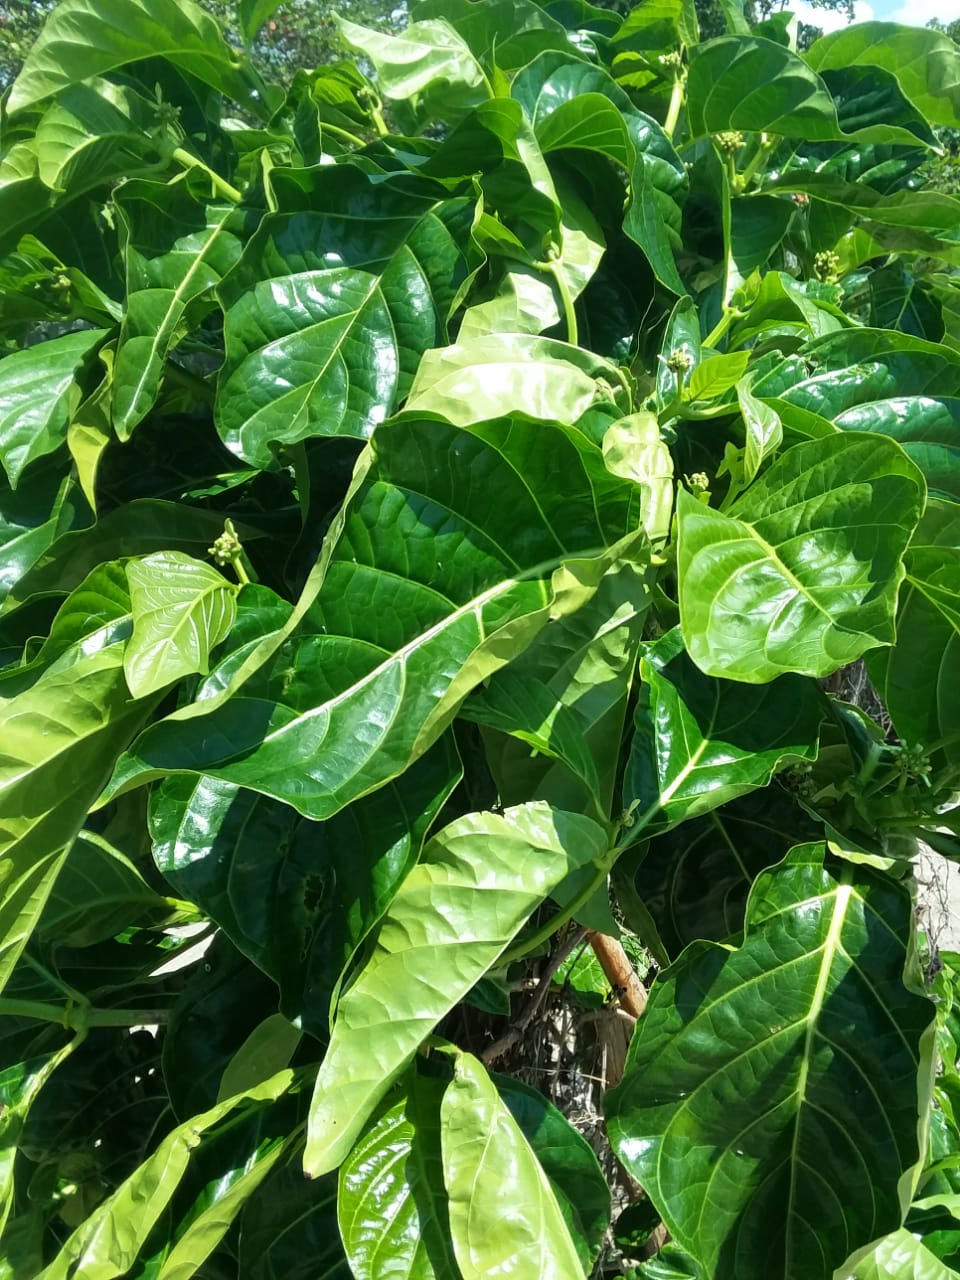
\includegraphics[height=2.60417in]{None.jpeg}
\caption{Morinda citrifolia (noni)\label{None}}
\end{figure}

\begin{figure}
\centering
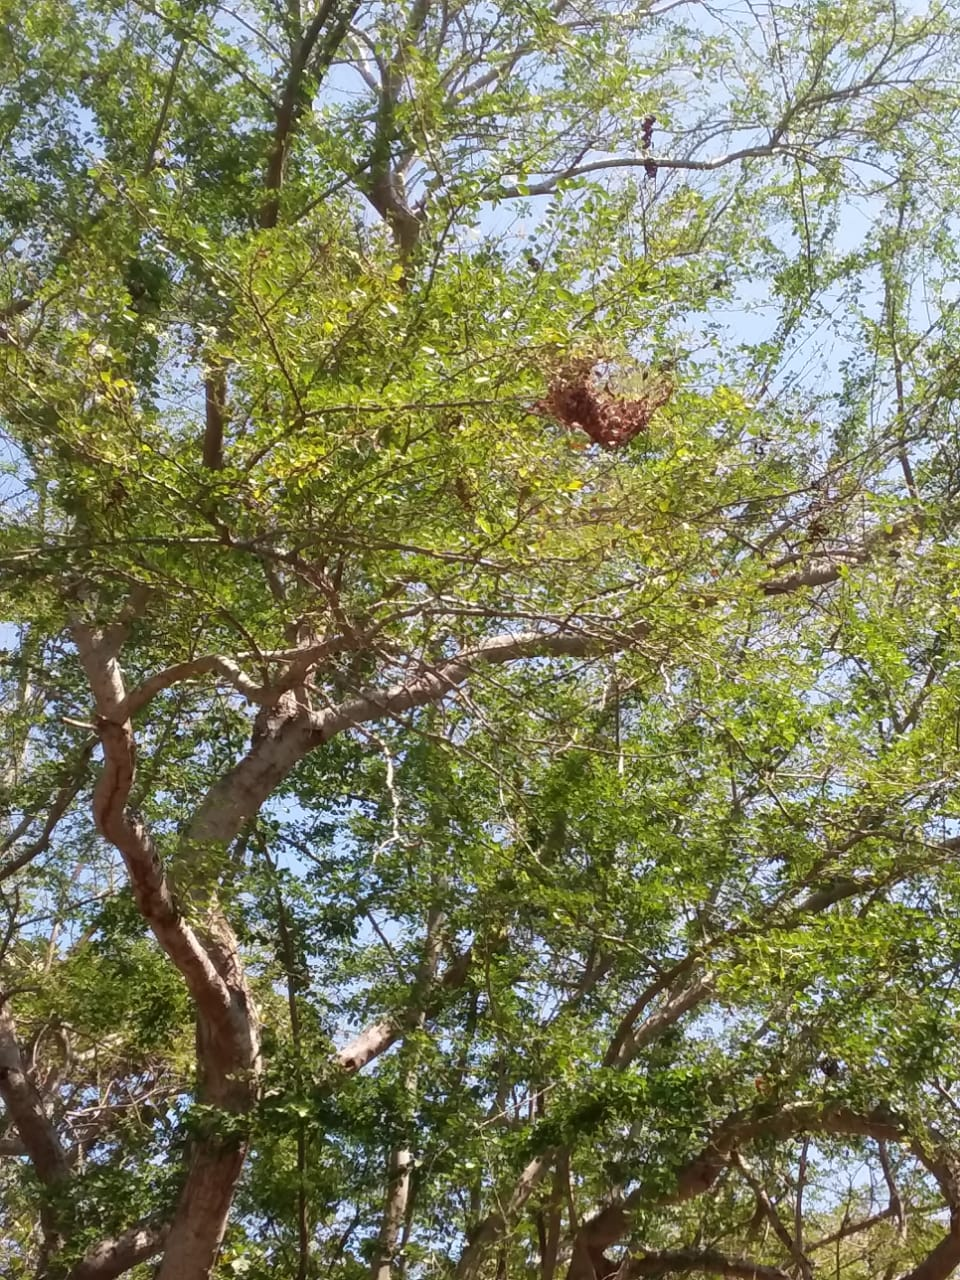
\includegraphics[height=2.60417in]{Gina.jpeg}
\caption{Pithecellobium (Gina)\label{gina}}
\end{figure}

\begin{figure}
\centering
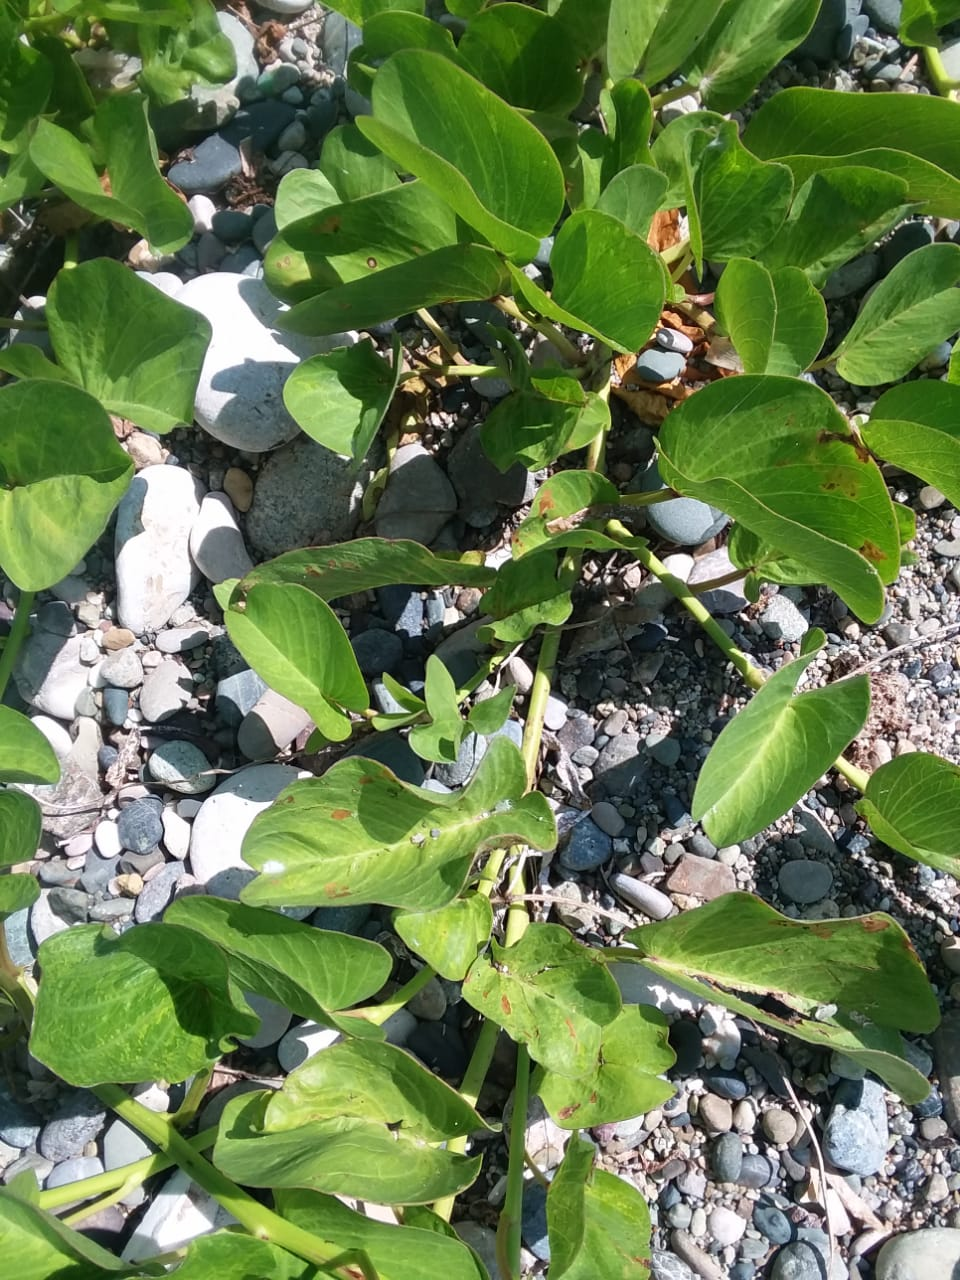
\includegraphics[height=2.60417in]{Ipomea.jpeg}
\caption{Ipomoea sp. \label{Ipomea}}
\end{figure}

\begin{figure}
\centering
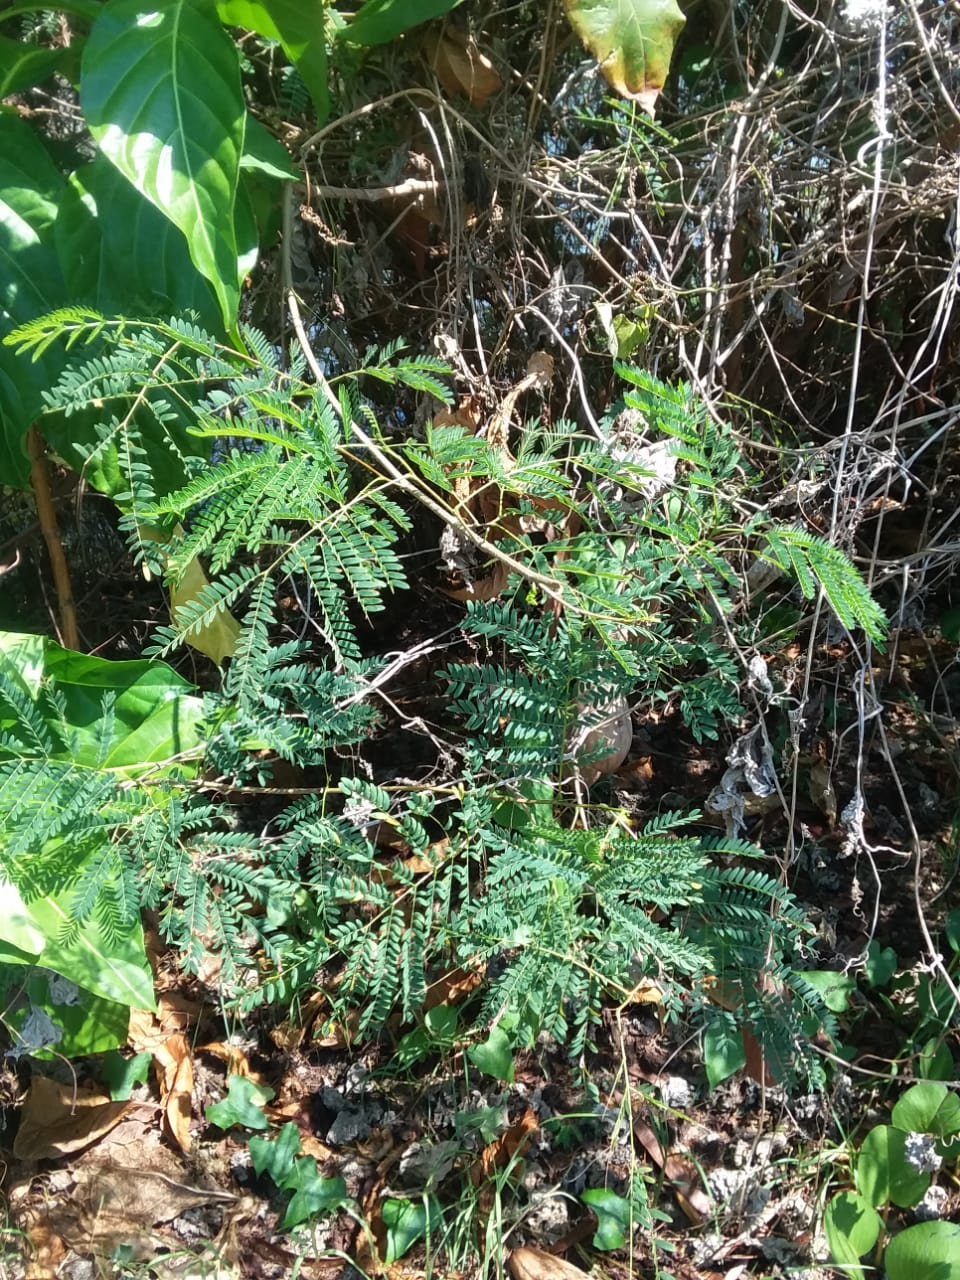
\includegraphics[height=2.60417in]{Limo.jpeg}
\caption{Lino \label{Limo}}
\end{figure}

\begin{figure}
\centering
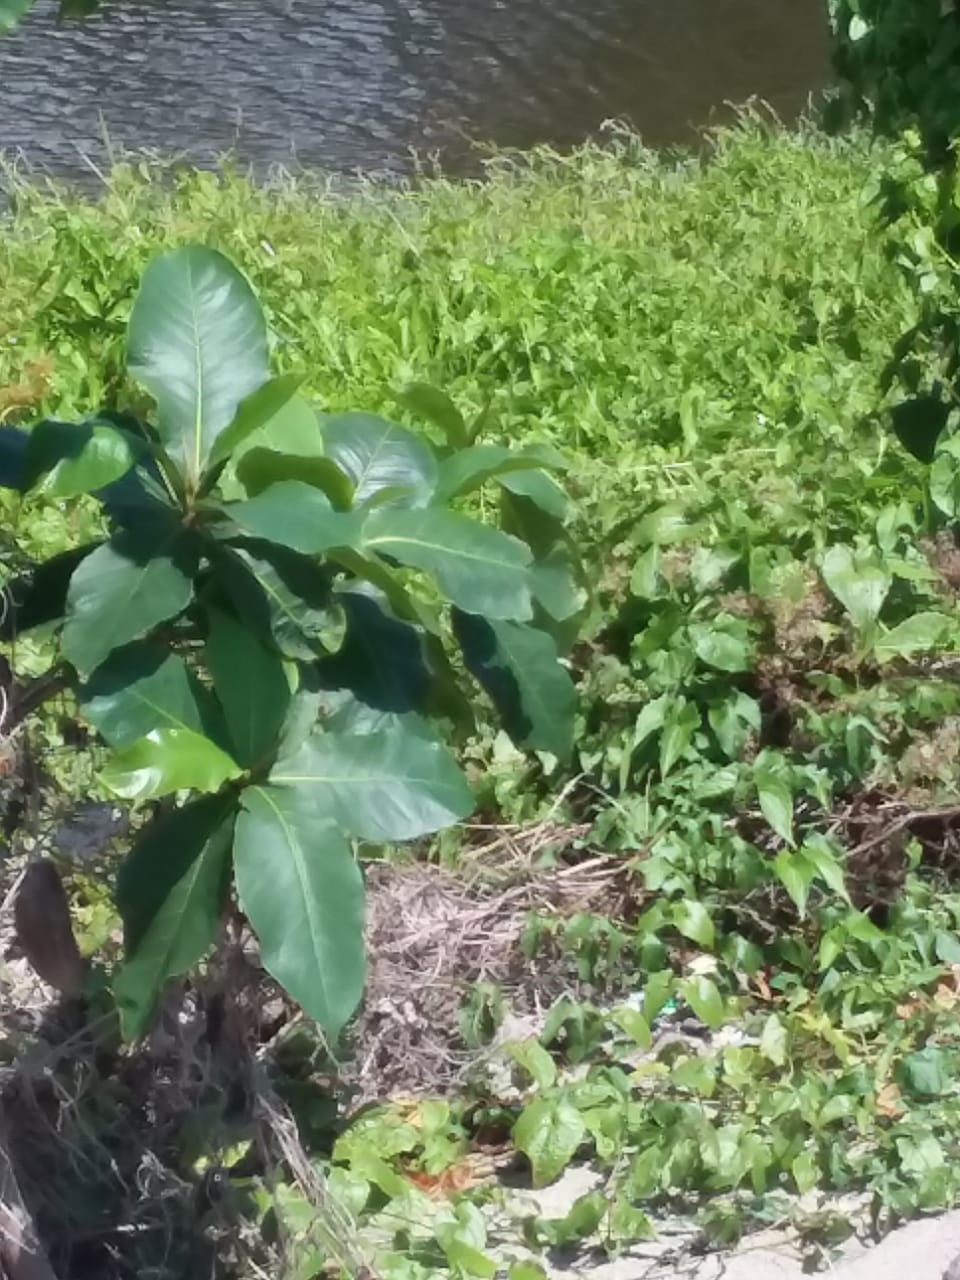
\includegraphics[height=2.60417in]{Almendra.jpeg}
\caption{Planta de cf.~almendra \label{Almendra}}
\end{figure}

Tras una revisión del conocimiento local expresado por lugareños, así
como por medio de información colectada en campo y de imágenes
satelitales, se hipotetiza que esta playa ha experimentado cambios en el
trazado de su línea de costa durante los últimos 6 años. Asimismo,
también se hipotetiza que existe una sustancial variabilidad espacial de
la inclinación y la concavidad del perfil de playa. Igualmente, se
formula la hipótesis de que la variabilidad observada en la distribución
de la granulometría de los sedimentos de la playa se debe se atribuye a
la relación del litoral con la desembocadura del arroyo Rolón.
Finalmente, también se hipotetiza que el beachrock encontrado en esta
playa podría atribuirse a descargas locales carbonatadas, posiblemente
de acuíferos o de fuentes superficiales. En tal sentido, para el
presente estudio, se formularon las siguientes preguntas:"

¿A qué se debe la diferencia de granulometria entre sedimentos en
distintos lugares de la playa?

¿Afectan los ciclones y los eventos de lluvias extremas no ciclónicas en
el trazado de línea de costa?

Si se han registrado cambios, ¿en qué año se registró el evento más
significativo que ha producido variación en el trazado de linea de
costa?

¿En qué parte de la playa se registran las mayores pendientes? ¿Por qué?

¿Por qué el Beachrock se localiza en el centro? ¿De qué está compuesto?

\section{Metodología}\label{metodologuxeda}

Se realizó una extensa revisión bibliográfica para conocer aspectos
geológicos y geomorfológicos sobre las costas de Najayo, así como para
situar el estado de conocimiento sobre esta poco reconocida localidad.

Para el estudio se aplicaron diversos métodos y se utilizaron varios
materiales, entre los cuales se incluyen: descripción general de la
costa, recogida de muestras de clastos, anotaciones, colecta de
coordenadas de precisión submétrica, compilación de líneas de costa
históricas mediante teledetección y análisis de cambio, realización de
vuelo con drone, generación ortofotografías y restitución
fotogramétrica.

Para la descripción general de la costa se colectaron muestras de
sedimentos a lo largo de la playa a intervalos regulares de
aproximadamente 70 metros. Se recogió un número máximo de cinco muestras
en lugares diferentes de la playa, tanto en la berma como en la ribera.
En cada espacio seleccionado se le asignaron un código para identificar
las muestras (ver figura \ref{mismuestrass}). Las tres localidades
occidentales se situaban cerca de la desembocadura del arroyo Rolón, y
las dos del extremo oriental, próximas a las costas acantiladas. Se
procedió a medir con una regla el largo y ancho de varios clastos
escogidos. Descartando aquellos con un tamaño inferior a 10 mm.

\begin{figure}
\centering
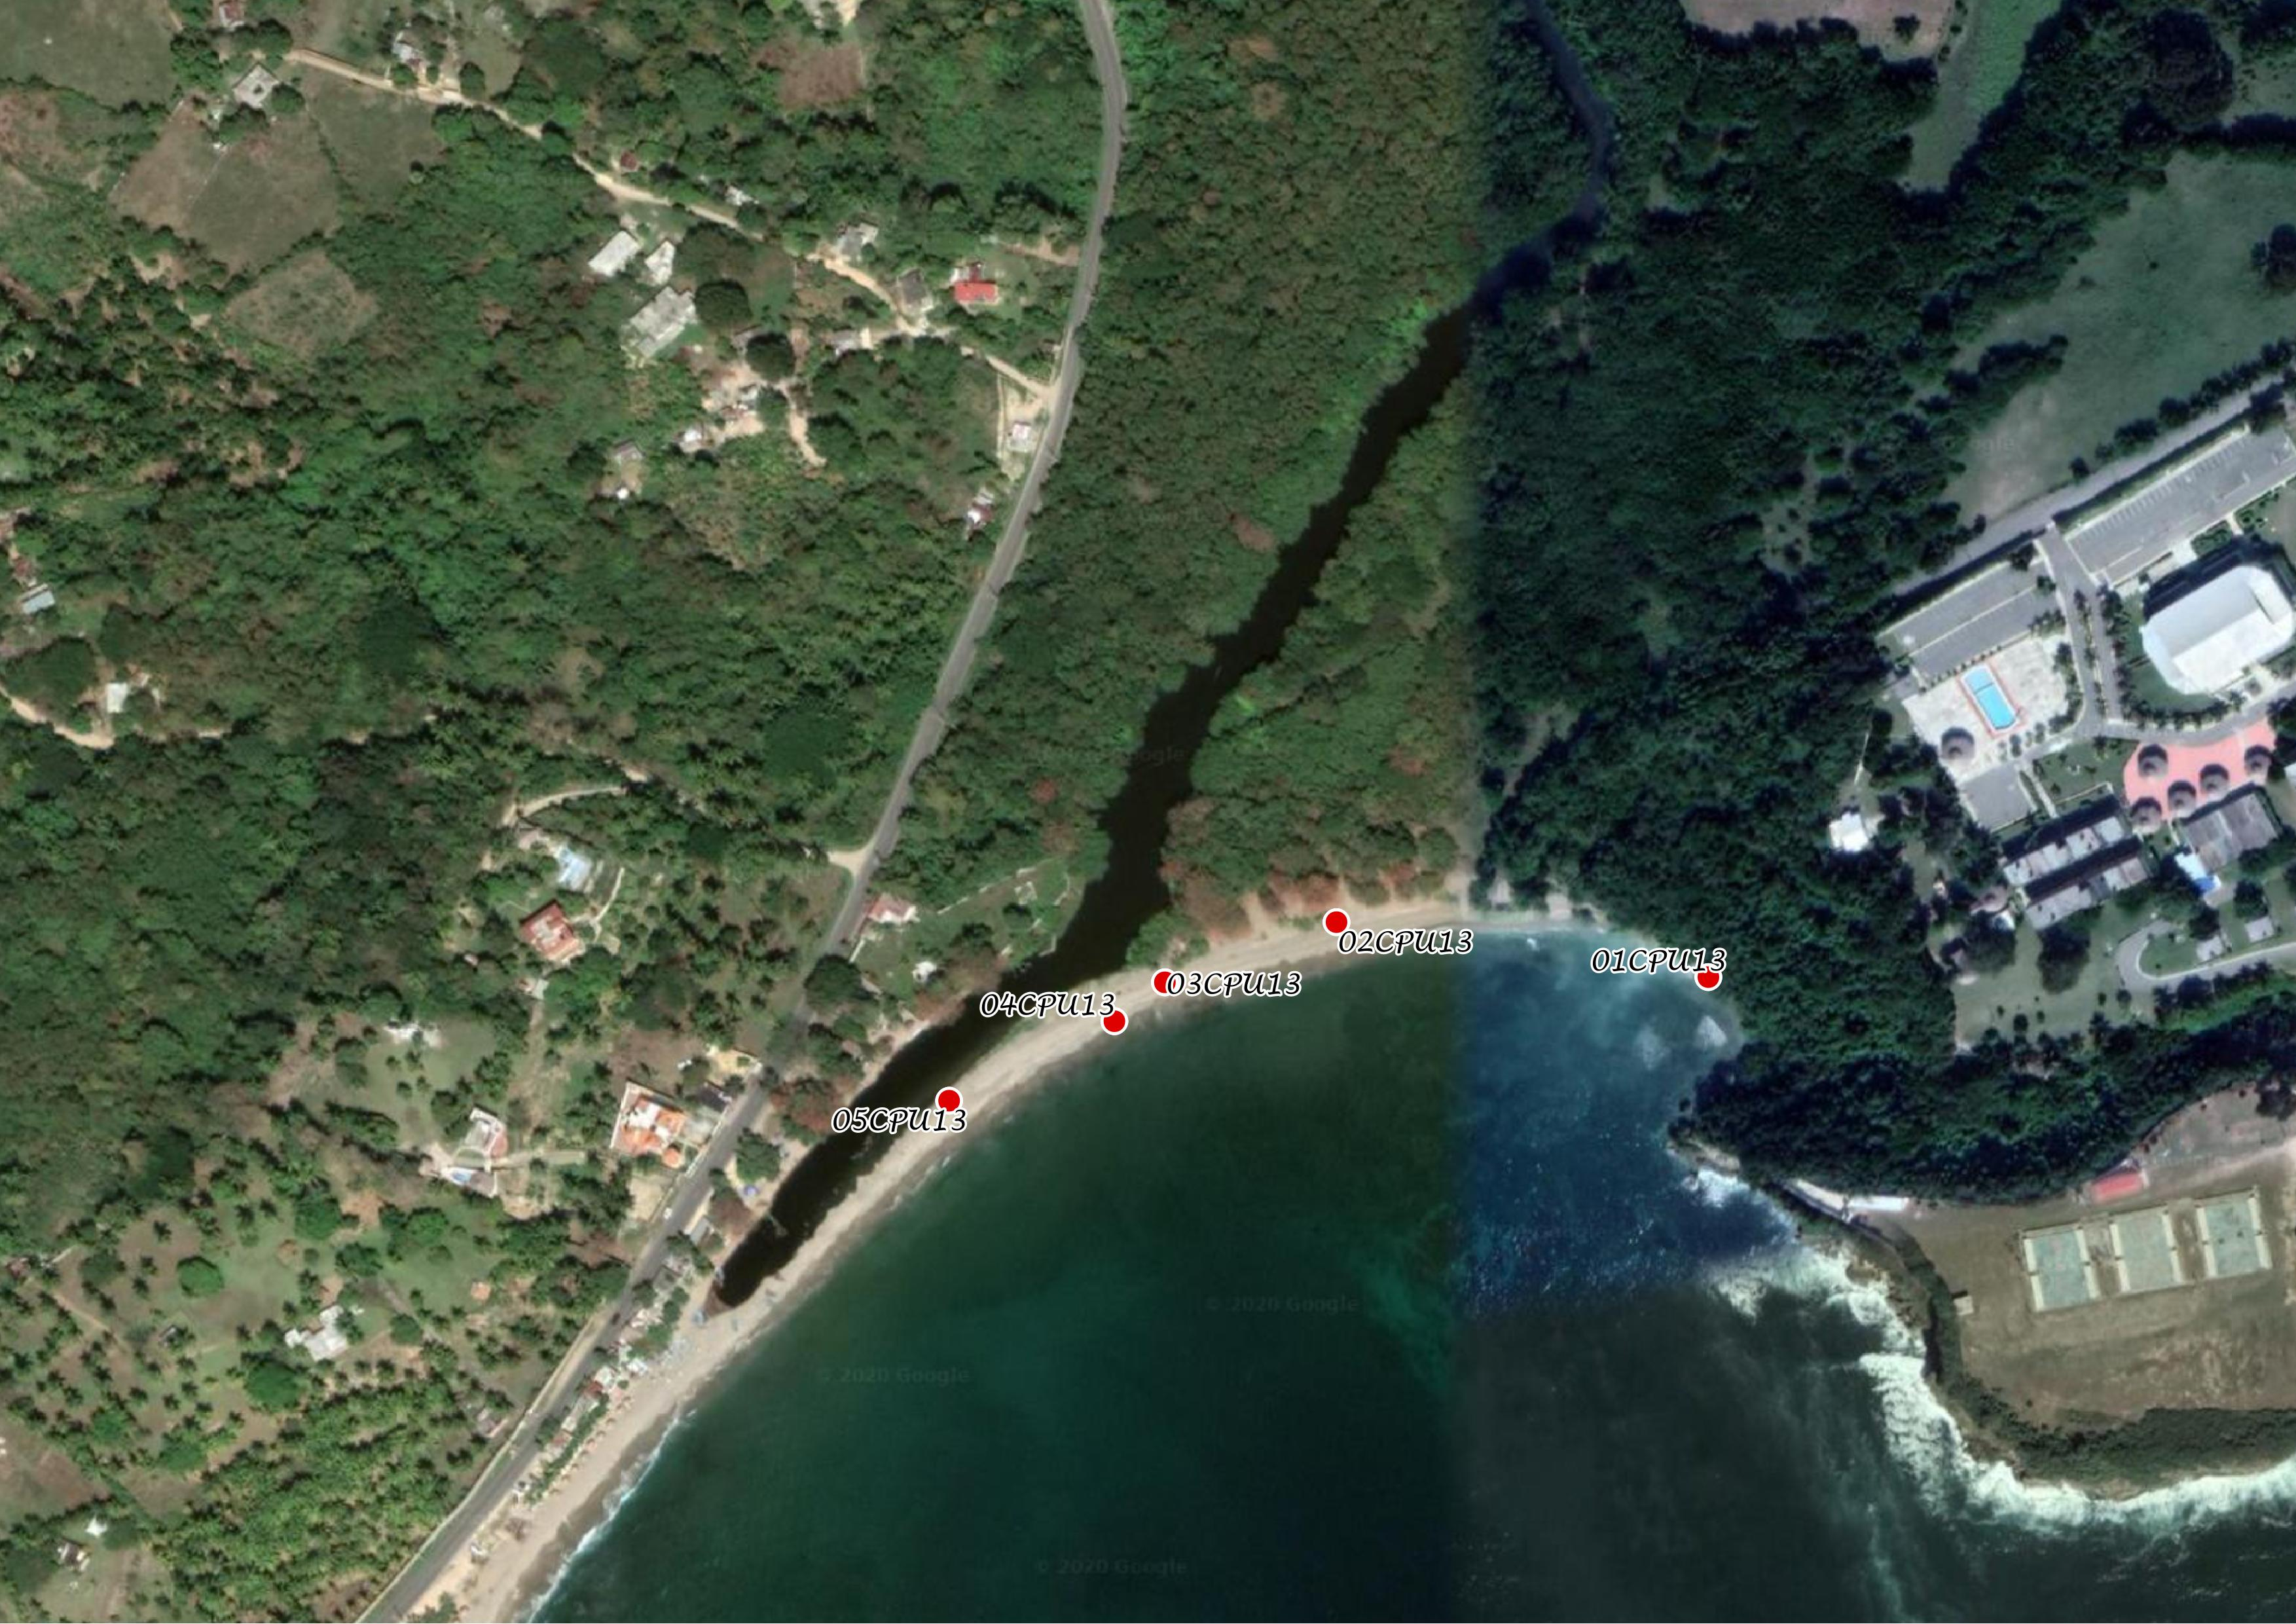
\includegraphics[height=3.12500in]{MUESTRASS.jpg}
\caption{Localización de los puntos de colecta \label{mismuestrass}}
\end{figure}

Para colectar sedimentos se utilizaron bolsas Whirl Pak de 540 ml(18oz),
4.5 pulgadas de ancho por 9 de largo, sobre las cuales se anotó con
tinta indeleble, código y fecha de colecta. Con la ayuda de la
aplicación ODK Collection se completó un formulario con los datos
referentes a las coordenadas,código de muestra, hora de colecta, fecha,
localidad y dueño de muestra.

Para fines de obtener coordenadas precisas se marcaron con pintura en
aerosol siete puntos en orden numérico a lo largo de la playa, y
utilizando un receptor de navegación satelital con tecnología RTK, se
obtuvo las coordenadas exactas de los lugares marcados.

Para analizar los cambios de trazado de la linea de costa, se compilaron
imagenes satelitáles de Landast 8 de los años 2013 a 2019, se usaron
para la detección de cambios ocurridos entre años pasados y la
actulidad. Para llevar a cabo el análisis de las modificaciones, fue
necesario delimitar la linea costera de la playa utilizando la
herramienta CoastSat (Vos, Splinter, Leaman, \& ianlturner, 2019). Estas
demarcaciones fueron limpiadas y hechas en Qgis (ver figura
\ref{lineas_najayo}).

\begin{figure}
\centering
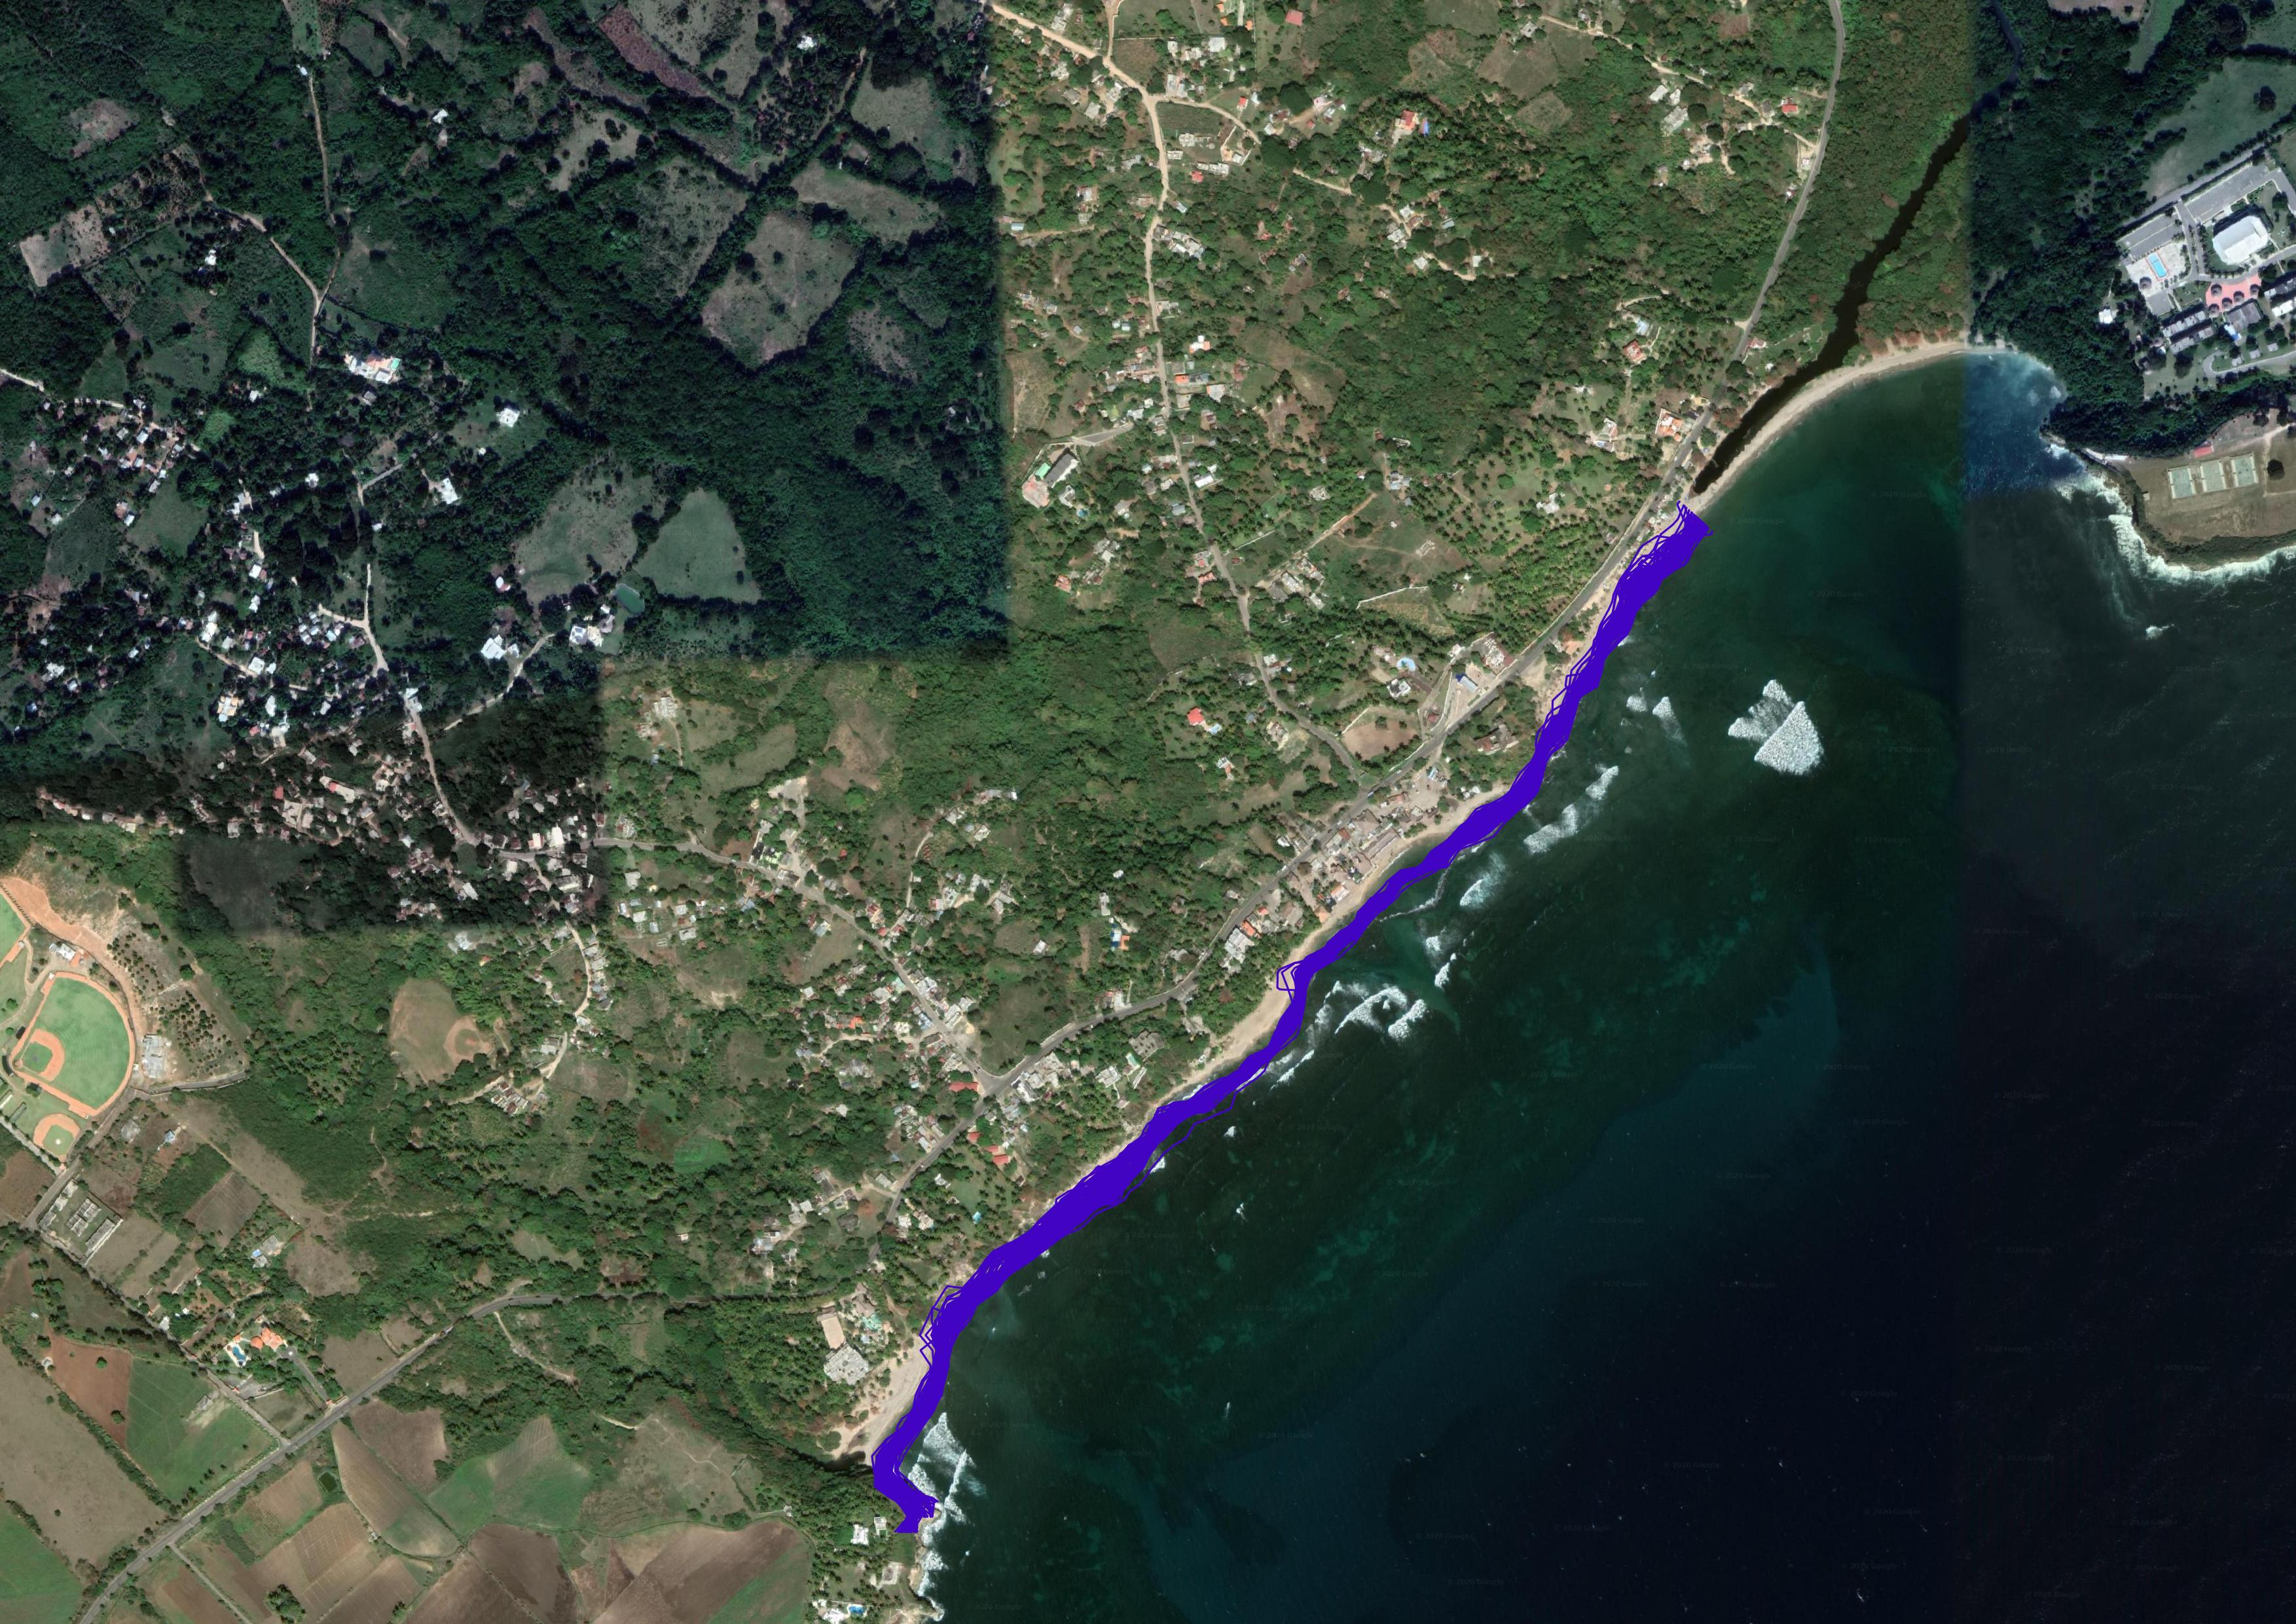
\includegraphics[height=3.12500in]{lineas_najayo.jpg}
\caption{Mapa de líneas de costa extraídas mediante CoastSat (ver texto)
\label{lineas_najayo}}
\end{figure}

Empleando el método de transectos lineales se recolectó información del
cambio dinámico que tiene el litoral en un periodo de siete años cada
tres meses. Se hacen trazados perpendiculares a la costa en la imágen, y
con las delimitaciones del litoral se toma una linea de referencia, se
estima la distancia entre ella y otra linea cualquiera. Finalmente,
tanto los transectos como las líneas fueron analizadas en R utilizaron
el script RCoastSat (Batlle, 2020), el cual produjo resultados gráficos
que facilitaron la interpretación.

Para responder las preguntas sobre pendiente y su distribución a lo
largo de la línea de costa, se realizó un vuelo con drone a lo largo de
la playa. De esta manera fueron tomadas imágenes aéreas con un drone
cuadrictéro modelo DJI Phantom 4, que cubrieron toda el área de la
costa. Para la correcta generación de ortofotografías y la restitución
fotogramétrica, se utilizaron coordenadas adquiridas con el sistema de
navegación mencionado, las cuales alimentaron el flujo de trabajo del
paquete OpenDroneMap.

Usando el DSM generado en OpenDroneMap y transectos en QGIS, con
herramientas visuales (Profile Tool en Qgis) mediante programación en R
para análisis por lote (Batlle, 2020) se generaron perfiles de playa.
Estas herramientas generan gráficos de perfil de elevación que muestran
la pendiente, una tabla de datos asociados, así como cálculos de
concavidad de perfil.

\section{Resultados}\label{resultados}

Los datos fueron agrupados en tres secciones de acuerdo, siguiendo los
temas formulados en el estudio: granulometría, cambios de trazado de la
línea de costa y perfiles de playa.

\subsection{Granulometría}\label{granulometruxeda}

Con las muestras ya recolectadas se procede a realizarse un análisis
granulométrico tomando medidas del largo y ancho de un total de 50
clastos. El estudio comparativo fue realizado contrastando las
mediciones de los clastos en dos unidades bien diferenciadas:berma
costera y frente de playa (incluyen ribera) n dos unidades
geomorfológicas berma costera y la ribera (ver figura
\ref{ab_por_muestras}).

\begin{figure}[H]
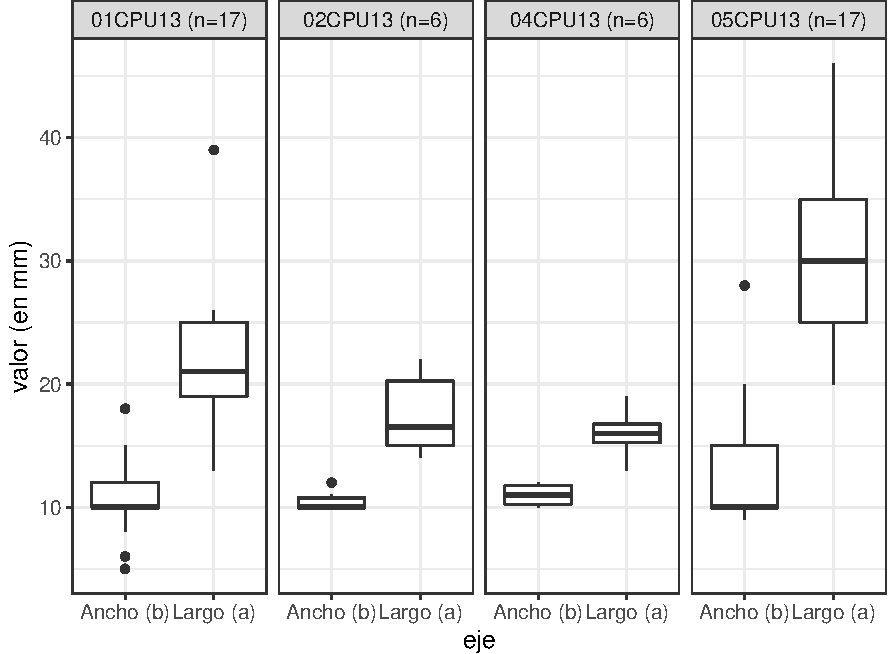
\includegraphics{manuscrito_files/figure-latex/unnamed-chunk-1-1} \caption{\label{ab_por_muestras}Dimensiones largo/ancho según muestras}\label{fig:unnamed-chunk-1}
\end{figure}

En la muestra de 01CPU13 (perteneciente a berma costera oriental) fueron
medidos 17 clastos con un promedio de tamaño entre 10 mm a 18 mm de
ancho, y 18 mm a 25 mm de largo y una mediana de 22 cm de largo. Se
identifican que dos clastos medidos en esta muestra tenían un ancho de
04 y 05 mm más pequeño que la mayor parte y solo uno con una dimensión
en 18 mm. En cambio se verifica un elemento con 39 mm de largo.

La segunda muestra colectada 02CPU13 se localiza en la berma central de
duna, se midieron seis elementos de los cuales el promedio en ancho es
de 10 a 12 mm y el largo de 15 a 20 mm. En esta colecta el 75\% de los
clastos mide menos de 20 mm de ancho y largo.

La cuarta muestra 04CPU13 se ubica frente al antiguo canal del arroyo
Rolón perteneciente a la ribera, se tomaron mediciones de 6 sedimentos,
cuyos resultados dieron una mediana de 11mm para ancho y 16 mm para
ancho. Todos midieron por debajo de 20 mm siendo estos los clastos más
pequeños de todos los recolectados.

La última muestra colectada llamada 05CPU13 se encuetra en la berma
occidental de la playa, en total se midieron 17 elementos. El rango de
valores se encuentra entre los 10 a 20 mm en ancho con solo un valor
atípico de 28 mm. En cambio la media en el largo fue de 25 mm a 35 mm,
es decir que un 50\% de los sedimentos media entre ese rango de valor.

\begin{figure}[H]
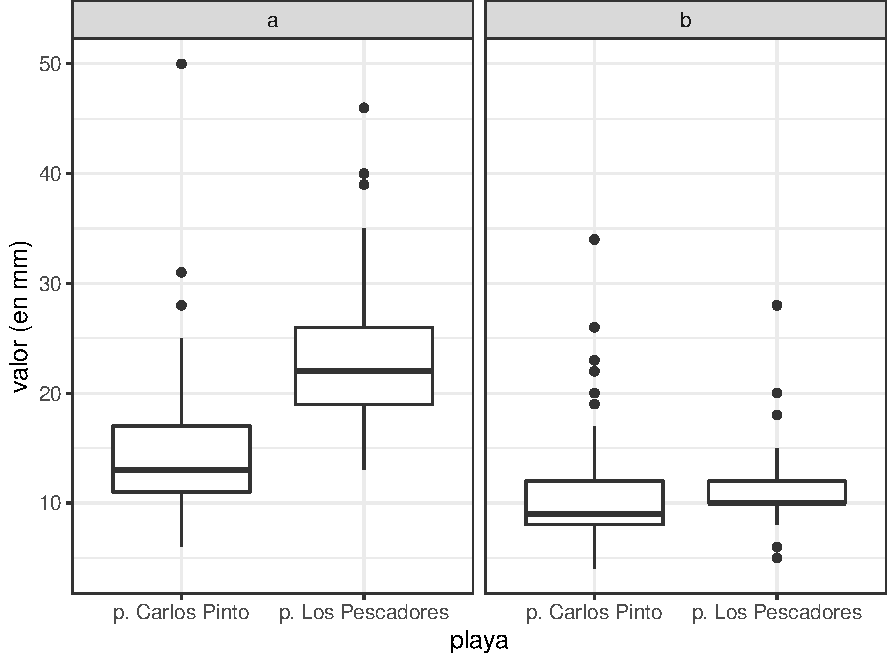
\includegraphics{manuscrito_files/figure-latex/unnamed-chunk-2-1} \caption{\label{ab_por_playas}Dimensiones largo/ancho según playas}\label{fig:unnamed-chunk-2}
\end{figure}

Se identifica una variación del tamaño de sedimentos en cada muestra de
las dos playas, donde se presentan valores más grandes tanto en ancho
como largo en la playa los Pescadores. En cambio en la playa Carlos
Pinto los clastos tienen un promedio menor en ambas dimensiones.

Los patrones correspondientes al eje largo en la laya Carlos Pinto miden
menos de 11mm en el 25\% de sus clastos, menos de 14 mm en el 50\% y no
superaban los 18 mm en un 75\% de sus elementos. En esta misma variable
en la playa los pescadores más del 50\% de los clastos superaban los 20
mm. En la variable ancho los clastos poseen un promedio de ente 9 a 12
mm en la playa Carlos Pinto, destacandose algunos valores atípicos. En
la otra playa un 75\% tienen un ancho de menos de 15 mm (ver figura
\ref{ab_por_playas}).

\subsection{Cambios de trazado de la línea de
costa}\label{cambios-de-trazado-de-la-luxednea-de-costa}

En cuanto al análisis de los cambios de trazado de la línea de costa, se
tomó como referencia una la línea del año 2013. La intersección entre el
transecto y cada linea que tiene asociada se forma un punto que contiene
un valor de fecha. El total de transectos trazados fueron 15, tomados
desde la desembocadura del arroyo Rolón hasta unos 10 metros al oeste.
Los presentados en azul representan el nivel de retirada del mar, de
modo que, una progradación de la costa y los de color marrón representan
el avance del mar hacia tierra (ver figuras \ref{transectosdplaya1},
\ref{transectosdplaya2} y \ref{transectosdplaya3}). Con esta información
se muestra si hay evidencia de retrogradación, progradación o por
defecto estacionaliddad en un periodo de siete años. A forma de cuadro
se realizan descripciones de los cambios por trimestre de cada año, se
observa que entre septiembre y diciembre de todos los años la
transgresión marina es más notable que en otros meses, por el contrario,
los meses de marzo a junio el hay una regresión marina de escasos metros
(ver figuras \ref{transectosdecambiocosta} y \ref{transectosNayajo}).

\begin{figure}
\centering
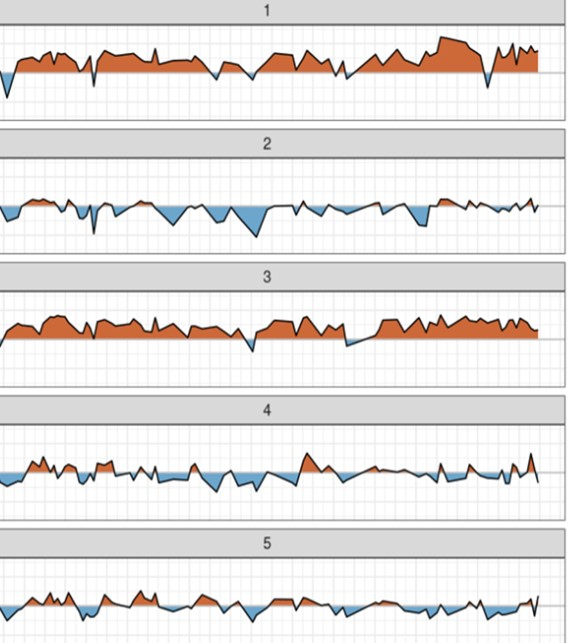
\includegraphics[height=5.20833in]{Rcoast_transectos1.jpg}
\caption{Cambios de trazado en los transectos 1 al 5, playa los
pescadores\label{transectosdplaya1}}
\end{figure}

\begin{figure}
\centering
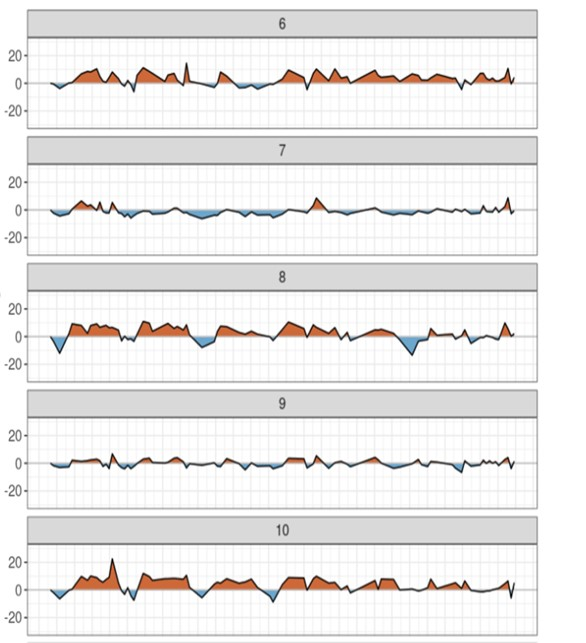
\includegraphics[height=5.20833in]{Rcoast_transectos2.jpg}
\caption{Cambios de trazado en los transectos 6 al 10, playa los
pescadores\label{transectosdplaya2}}
\end{figure}

\begin{figure}
\centering
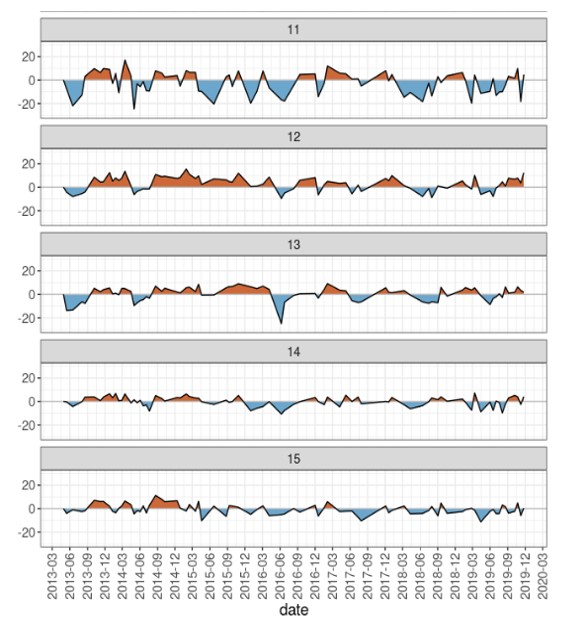
\includegraphics[height=5.20833in]{Rcoast_transectos3.jpg}
\caption{Cambios de trazado en los transectos 6 al 10, playa los
pescadores\label{transectosdplaya3}}
\end{figure}

\begin{figure}
\centering
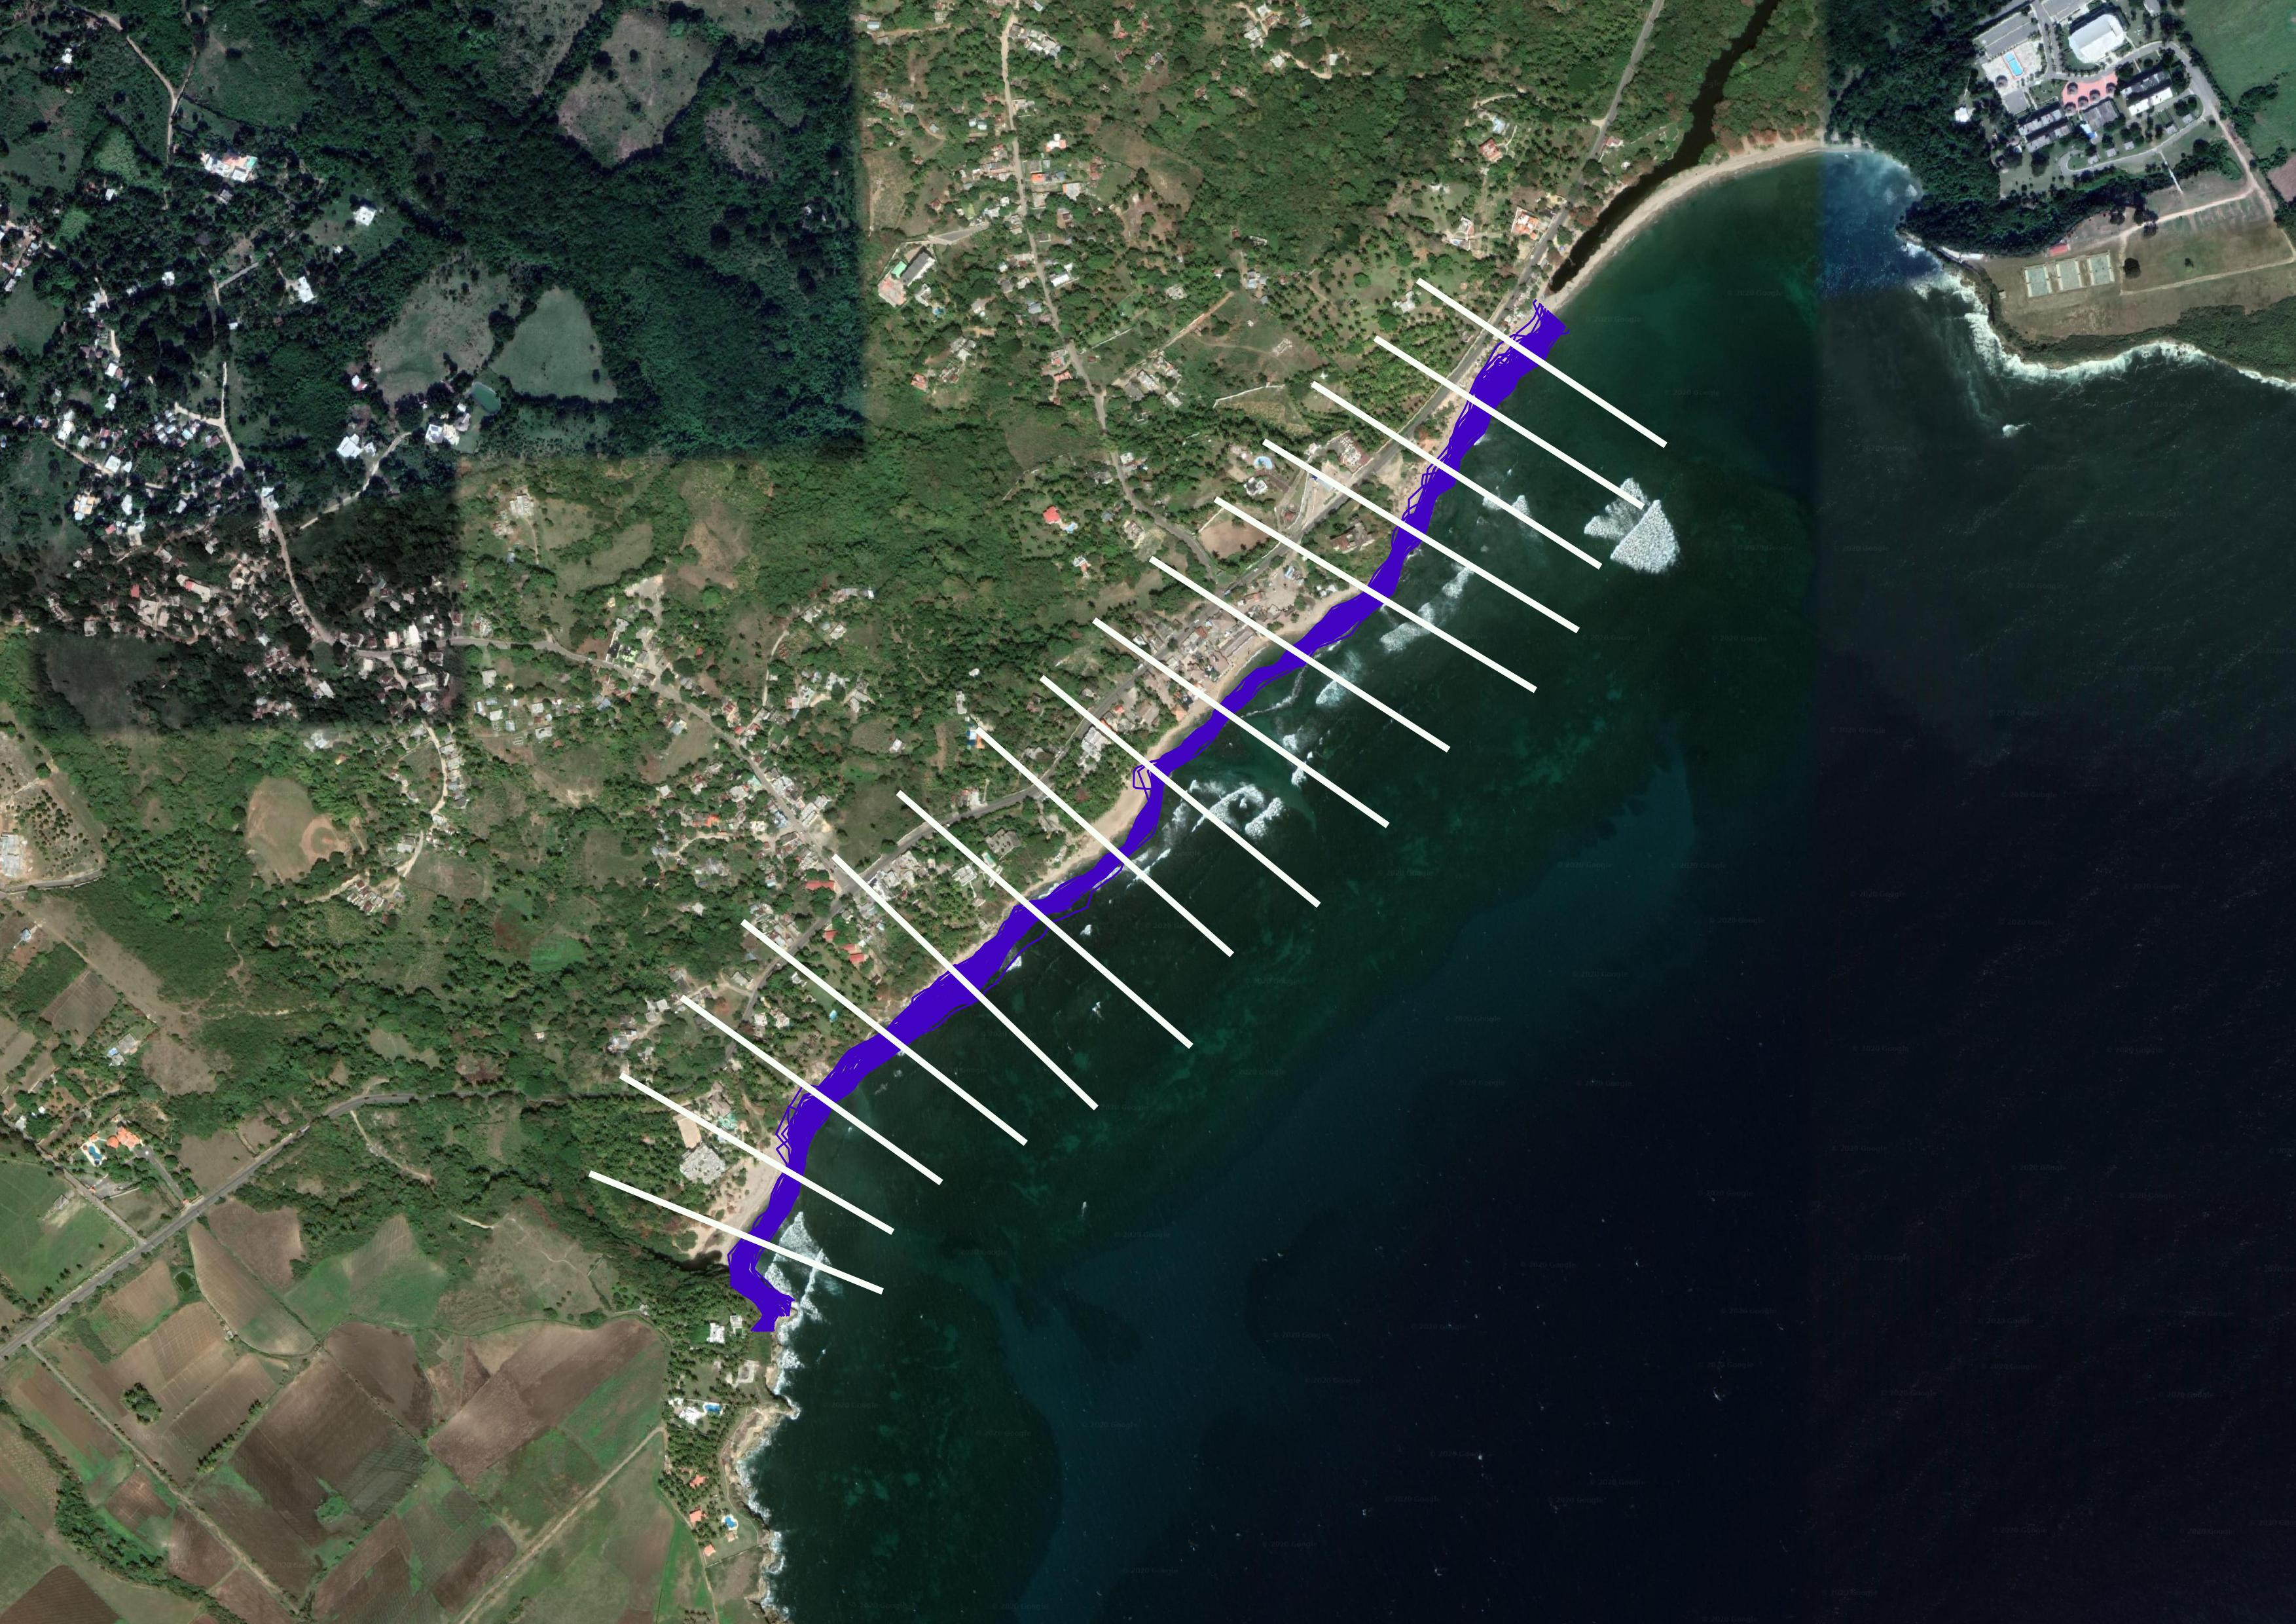
\includegraphics[height=4.16667in]{transectosdplaya.jpg}
\caption{Digitalización de transectos de playa los
pescadores\label{transectosdecambiocosta}}
\end{figure}

\begin{figure}
\centering
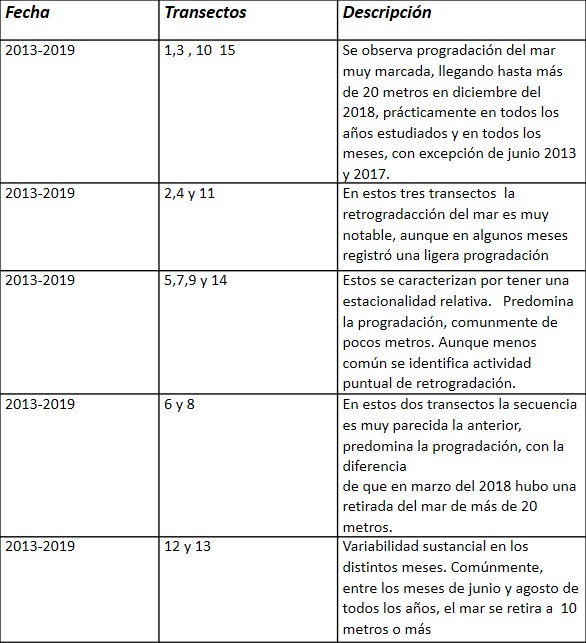
\includegraphics[height=5.20833in]{Descripcion_transectos.jpg}
\caption{Resumen de los cambios en la línea de costa
\label{transectosNayajo}}
\end{figure}

\subsection{Perfil de playa}\label{perfil-de-playa}

Se extrajeron perfiles de playa de un modelo digital de superficie,
donde se muestra la generación 20 perfiles topográficos divididos en 4
plots de 5 paneles cada uno de la playa de Los pescadores. Las
observaciones de los paneles indican que se mantiene una tendencia de
bajada a medida que se aproxima al occidente del litoral, entre los
transectos 6 a 12 la pendiente queda casi completamente tendida llegando
a 0.5 metros en el transecto 12, a partir del transecto 13 la pendiente
se vuelve ligeramente más pronunciada, llegando alcanzar valores
superiores a 2.5 metros en el transecto 17 (ver figuras
\ref{transectos-mapa}, \ref{transectos-perfil1},
\ref{transectos-perfil2}, \ref{transectos-perfil3} y
\ref{transectos-perfil4}).

En estos grupos de subtipos de transectos a escalas iguales entre
paneles del mismo plot (no vertical exaggeration), usan los mismos
límites para sus ejes entre paneles (transectos), los valores para el
eje x van desde 0 a 3.5 metros, el eje y es igual. Estos gráficos son
útiles para saber, por ejemplo, cuáles transectos llegan al nivel cero
arbitrario y cuáles no, así como para comparar cuáles tienen mayor
desplazamiento horizontal y cuáles tienen menos.

\begin{figure}
\centering
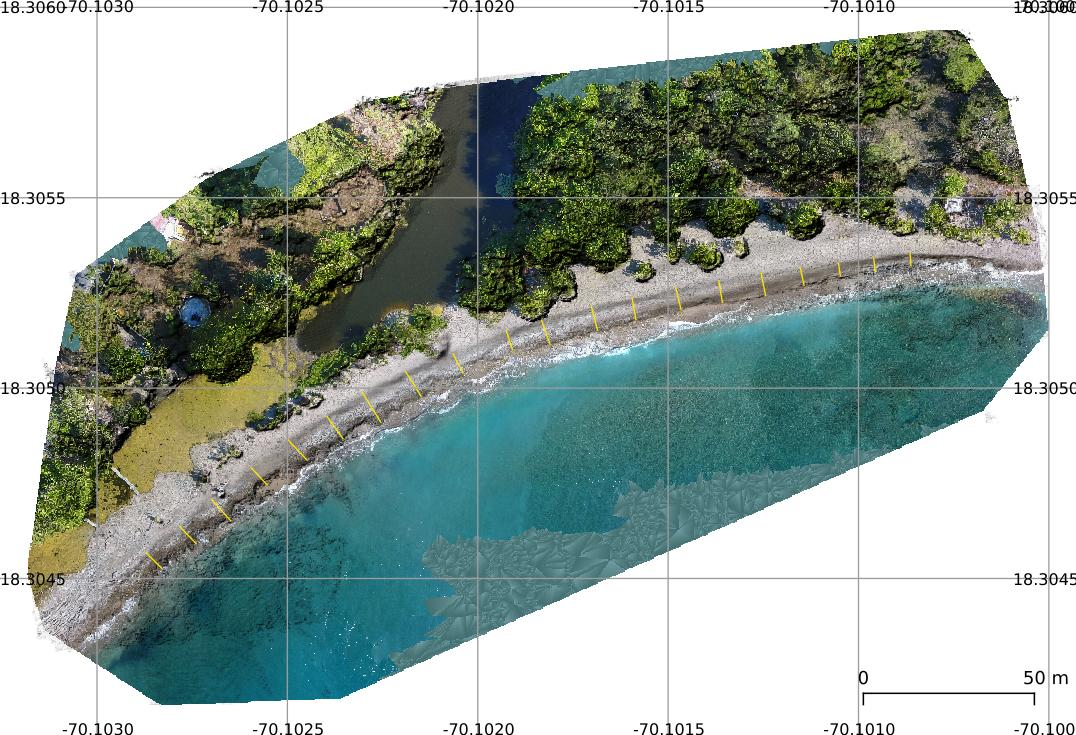
\includegraphics[height=3.12500in]{transects-qgis.jpg}
\caption{Mapa de transectos para generar perfiles de
playa\label{transectos-mapa}}
\end{figure}

\begin{figure}
\centering
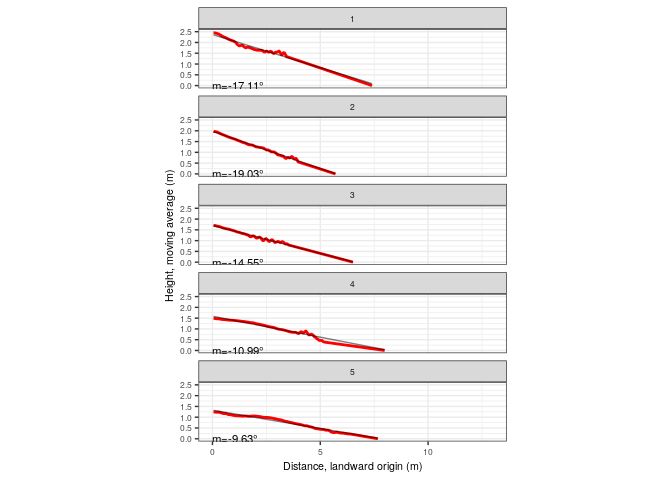
\includegraphics[height=8.33333in]{panels-1.png}
\caption{Pendientes de los transectos 1 a 5 (cortes sin exageración
vertical) \label{transectos-perfil1}}
\end{figure}

\begin{figure}
\centering
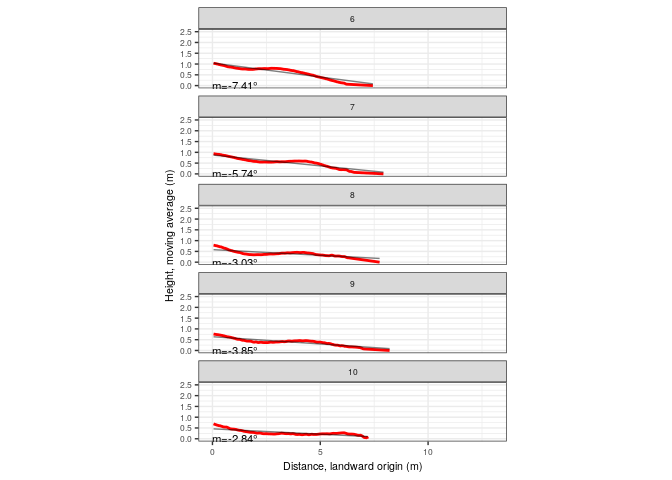
\includegraphics[height=8.33333in]{panels-2.png}
\caption{Pendientes de los transectos 6 a 10 (cortes sin exageración
vertical) \label{transectos-perfil2}}
\end{figure}

\begin{figure}
\centering
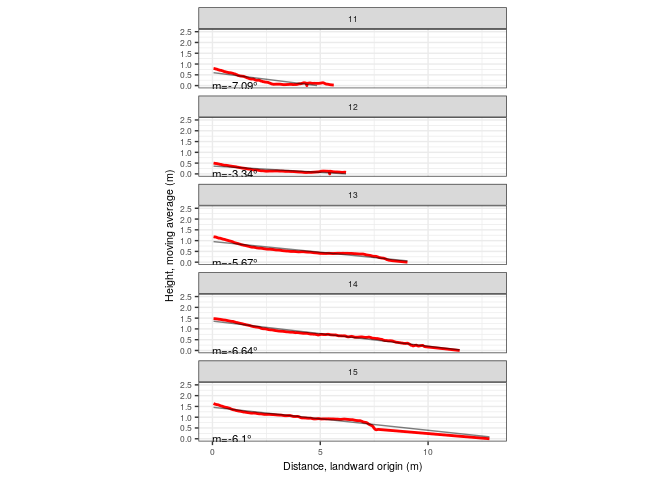
\includegraphics[height=8.33333in]{panels-3.png}
\caption{Pendientes de los transectos 11 a 15 (cortes sin exageración
vertical) \label{transectos-perfil3}}
\end{figure}

\begin{figure}
\centering
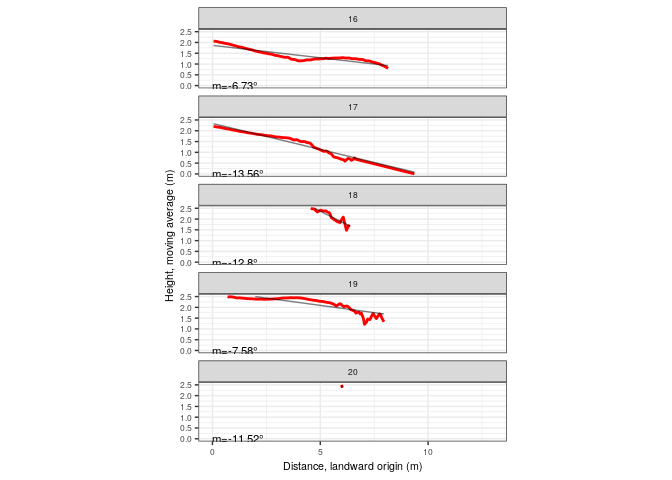
\includegraphics[height=8.33333in]{panels-4.png}
\caption{Pendientes de los transectos 16 a 20 (cortes sin exageración
vertical) \label{transectos-perfil4}}
\end{figure}

\begin{figure}
\centering
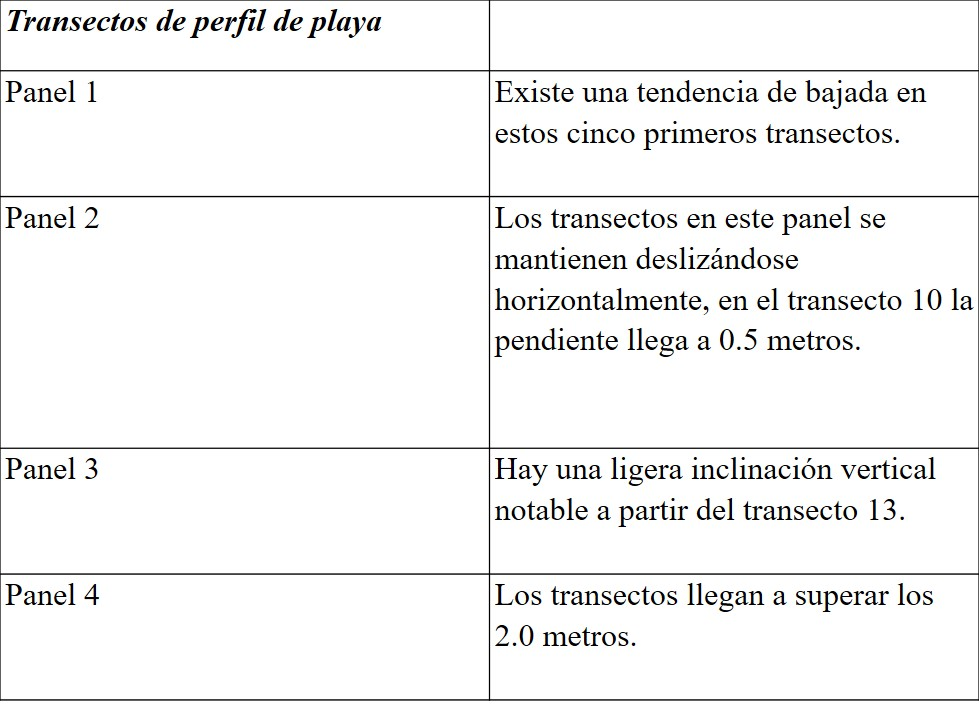
\includegraphics[height=4.16667in]{Descripcion_paneles.jpg}
\caption{Descripción de transectos \label{transectos-playa}}
\end{figure}

\section{Discusión}\label{discusiuxf3n}

Se formularon diversas hipótesis para las preguntas planteadas. Para la
pregunta sobre la diferencia de tamaños de los clastos en las dos playa,
se sostiene que los sedimentos del continente fueron arrastrados por el
arroyo Rolón de manera constante hasta ser depositados en la costa de la
playa los pescadores. En cambio, el arroyo de agua dulce que desembocaba
en la playa de Carlos Pinto se vió afectado por un estancamiento por la
acumulación de sedimentos. Hay registro de que el cauce del arroyo Rolón
es más amplió y su cuenca es mayor que la de arroyo de agua dulce, por
otro lado, la deriva predominante viene de los vientos del nordeste, que
con el oleaje y el cambio brusto de refracción produce acumulación en la
ensenada en la playa los pescadores, mientras que en Carlos Pinto este
oleaje llega ya reflactado lo hace que su erosión y posterior
acumulación sea mucho menor. Esto puede explicar la variación de tamaño
de sedimentos en ambas playas.

De acuerdo con (Carranza-Edwards, 2010) la velocidad de erosión en las
playas puede variar considerablemente en el espacio y tiempo, así, los
huracanes pueden tener una respuesta inmedianta en la erosión de las
playas. En consideración a esto, el cambio más notable de progradación
del mar se registra en el trimestre de junio-septiembre del 2016,
periodo en el que superó los 20 metros de distancia, presuntamente por
el huracán Mathew de categoría cinco ocurrido en en septiembre del 2016.

Diversas investigaciones sostienen que el \emph{beachrock} de la playa
está compuesto por basalto, fósiles arrastrados, rocas alteradas,
tonalitas, calizas, rocas intrusivas fosilizada por carbonato de calcio
usual en la región sur de la Republica Dominicana y propio del periodo
pleistoceno. Todos estos materiales fueron depositados y empastados por
el carbonato del continente y otros arrastrasdos por el mar desde el
rio. Se localiza en el centro (entre punta y punta de la playa Najayo)
porque es donde afloran las calizas con mayor claridad.

Para concluir, la playa presenta un perfil de forma concava, teniendo
mayor pendiente es en la berma frente al Antiguo Canal del arroyo. El
transporte de sedimento desde el arroyo hasta llegar al mar generan una
acumulación de estos en esta parte de la berma.

\section{Agradecimientos}\label{agradecimientos}

En primer lugar quiero agradecer al profesor José Ramón Martinez Battle
del área de las ciencias geográficas de la Universidad Autónoma de Santo
Domingo por tener la iniciativa, propiciar las investigaciones y
facilitar las herramientas para este estudio.

También le agradezco a la facultad de Ciencias y la escuela de geografía
de la Universidad Autónoma de Santo Domingo por ser fuente de formación
de profesionales en esta área.

Por último agradezco a la estudiante de Ciencias Geográficas Ana Valera
por sumarse y ser de ayuda idónea en las investigaciones hechas en esta
playa.

\section{Información de soporte}\label{informaciuxf3n-de-soporte}

\ldots

\section{\texorpdfstring{\emph{Script}
reproducible}{Script reproducible}}\label{script-reproducible}

\begin{Shaded}
\begin{Highlighting}[]
\KeywordTok{library}\NormalTok{(jsonlite)}
\KeywordTok{library}\NormalTok{(tidyverse)}
\NormalTok{df <-}\StringTok{ }\NormalTok{jsonlite}\OperatorTok{::}\KeywordTok{fromJSON}\NormalTok{(}\StringTok{'Cantometría_3_results.json'}\NormalTok{, }\DataTypeTok{flatten =} \OtherTok{TRUE}\NormalTok{)}
\NormalTok{df }\OperatorTok\StringTok{ }\KeywordTok{filter}\NormalTok{(}\OperatorTok{!}\KeywordTok{grepl}\NormalTok{(}\StringTok{'^C2.*M1$|^AV.*$'}\NormalTok{, codigomuestra), }\KeywordTok{grepl}\NormalTok{(}\StringTok{'T23'}\NormalTok{, df}\OperatorTok{$}\NormalTok{fechahora)) }\OperatorTok\StringTok{ }\KeywordTok{unnest}\NormalTok{(clastos) }\OperatorTok\StringTok{ }\KeywordTok{View}\NormalTok{()}
\NormalTok{df  }\OperatorTok\StringTok{ }\KeywordTok{filter}\NormalTok{(}\OperatorTok{!}\KeywordTok{grepl}\NormalTok{(}\StringTok{'^C2.*M1$|^AV.*$'}\NormalTok{, codigomuestra), }\KeywordTok{grepl}\NormalTok{(}\StringTok{'T23'}\NormalTok{, df}\OperatorTok{$}\NormalTok{fechahora)) }\OperatorTok\StringTok{ }\KeywordTok{unnest}\NormalTok{(clastos) }\OperatorTok
\StringTok{  }\KeywordTok{select}\NormalTok{(}\StringTok{`}\DataTypeTok{Codigo de lugar}\StringTok{`}\NormalTok{=codigomuestra, }\StringTok{`}\DataTypeTok{Largo (a)}\StringTok{`}\NormalTok{=a, }\StringTok{`}\DataTypeTok{Ancho (b)}\StringTok{`}\NormalTok{=b) }\OperatorTok
\StringTok{  }\KeywordTok{group_by}\NormalTok{(}\StringTok{`}\DataTypeTok{Codigo de lugar}\StringTok{`}\NormalTok{) }\OperatorTok
\StringTok{  }\KeywordTok{mutate}\NormalTok{(}\StringTok{'Codigo de lugar n'}\NormalTok{=}\KeywordTok{paste0}\NormalTok{(}\StringTok{`}\DataTypeTok{Codigo de lugar}\StringTok{`}\NormalTok{, }\StringTok{' (n='}\NormalTok{, }\KeywordTok{length}\NormalTok{(}\StringTok{`}\DataTypeTok{Codigo de lugar}\StringTok{`}\NormalTok{), }\StringTok{')'}\NormalTok{)) }\OperatorTok
\StringTok{  }\KeywordTok{ungroup}\NormalTok{() }\OperatorTok\StringTok{ }\KeywordTok{select}\NormalTok{(}\OperatorTok{-}\StringTok{`}\DataTypeTok{Codigo de lugar}\StringTok{`}\NormalTok{) }\OperatorTok\StringTok{ }\KeywordTok{gather}\NormalTok{(eje, }\StringTok{`}\DataTypeTok{valor (en mm)}\StringTok{`}\NormalTok{, }\OperatorTok{-}\StringTok{`}\DataTypeTok{Codigo de lugar n}\StringTok{`}\NormalTok{) }\OperatorTok
\StringTok{  }\KeywordTok{ggplot}\NormalTok{() }\OperatorTok{+}\StringTok{ }\KeywordTok{aes}\NormalTok{(}\DataTypeTok{x =}\NormalTok{ eje, }\DataTypeTok{y =} \StringTok{`}\DataTypeTok{valor (en mm)}\StringTok{`}\NormalTok{) }\OperatorTok{+}\StringTok{ }\KeywordTok{geom_boxplot}\NormalTok{() }\OperatorTok{+}
\StringTok{  }\KeywordTok{facet_grid}\NormalTok{(}\OperatorTok{~}\StringTok{`}\DataTypeTok{Codigo de lugar n}\StringTok{`}\NormalTok{) }\OperatorTok{+}\StringTok{ }\KeywordTok{theme_bw}\NormalTok{() }\OperatorTok{+}
\StringTok{  }\KeywordTok{theme}\NormalTok{(}\DataTypeTok{text =} \KeywordTok{element_text}\NormalTok{(}\DataTypeTok{size =} \DecValTok{18}\NormalTok{))}



\NormalTok{Packages}
\KeywordTok{library}\NormalTok{(tidyverse)}
\KeywordTok{library}\NormalTok{(purrr)}
\KeywordTok{library}\NormalTok{(sf)}
\KeywordTok{library}\NormalTok{(RColorBrewer)}
\KeywordTok{library}\NormalTok{(raster)}
\NormalTok{Read the functions}
\NormalTok{funs <-}\StringTok{ }\KeywordTok{list.files}\NormalTok{(}\StringTok{'R'}\NormalTok{, }\DataTypeTok{pattern =} \StringTok{'*.R'}\NormalTok{, }\DataTypeTok{full.names =}\NormalTok{ T)}
\KeywordTok{map}\NormalTok{(funs, source)}
\NormalTok{atransprof <-}\StringTok{ }\KeywordTok{rtrans}\NormalTok{(}\StringTok{'data/perfil_los_pescadores.geojson'}\NormalTok{)}\CommentTok{#Digitized by Carolain, edited by geofis}
\NormalTok{## Reading layer `transectos_ortofotos' from data source `/home/jr/Documentos/git/BeachProfile/data/perfil_los_pescadores.geojson' using driver `GeoJSON'}
\NormalTok{## Simple feature collection with 20 features and 1 field}
\NormalTok{## geometry type:  LINESTRING}
\NormalTok{## dimension:      XY}
\NormalTok{## bbox:           xmin: 383443.4 ymin: 2024230 xmax: 383656.2 ymax: 2024320}
\NormalTok{## epsg (SRID):    32619}
\NormalTok{## proj4string:    +proj=utm +zone=19 +datum=WGS84 +units=m +no_defs}
\NormalTok{rawDsm <-}\StringTok{ }\KeywordTok{raster}\NormalTok{(}\StringTok{'data/raw-dsm-pescadores.tif'}\NormalTok{)}
\NormalTok{dsm <-}\StringTok{ }\KeywordTok{thresholdRaise}\NormalTok{(}\DataTypeTok{rasterDsm =}\NormalTok{ rawDsm, }\DataTypeTok{threshold =} \OperatorTok{-}\FloatTok{44.1}\NormalTok{)}
\KeywordTok{plot}\NormalTok{(dsm)}
\KeywordTok{plot}\NormalTok{(}\KeywordTok{as_Spatial}\NormalTok{(transprof), }\DataTypeTok{add=}\NormalTok{T)}
\end{Highlighting}
\end{Shaded}

\begin{figure}
\centering
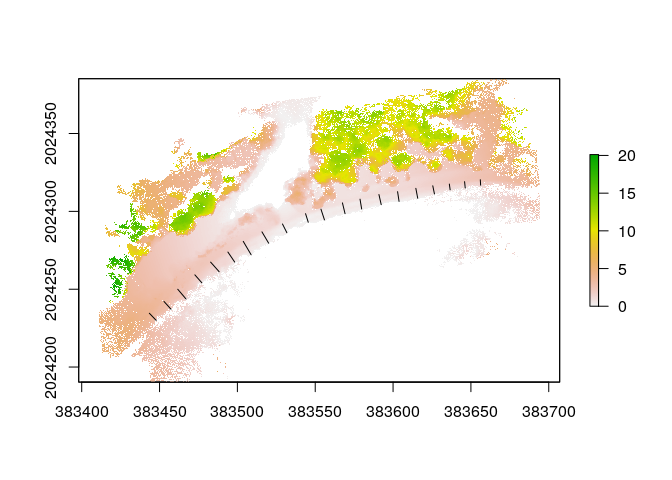
\includegraphics[height=3.12500in]{carolaint1.png}
\caption{\label{transectos-playa}}
\end{figure}

\begin{Shaded}
\begin{Highlighting}[]
\CommentTok{#ggplot of transects}
\NormalTok{cols <-}\StringTok{ }\KeywordTok{colorRampPalette}\NormalTok{(}\KeywordTok{brewer.pal}\NormalTok{(}\DecValTok{9}\NormalTok{,}\StringTok{'Set1'}\NormalTok{))(}\KeywordTok{nrow}\NormalTok{(transprof))}
\KeywordTok{ggplot}\NormalTok{() }\OperatorTok{+}
\StringTok{  }\KeywordTok{geom_sf}\NormalTok{(}\DataTypeTok{data =}\NormalTok{ transprof, }\DataTypeTok{color =}\NormalTok{ cols) }\OperatorTok{+}
\StringTok{  }\KeywordTok{scale_color_manual}\NormalTok{(}\DataTypeTok{values =} \KeywordTok{c}\NormalTok{(}\StringTok{'black'}\NormalTok{, }\StringTok{'orange'}\NormalTok{, }\StringTok{'blue'}\NormalTok{)) }\OperatorTok{+}
\StringTok{  }\KeywordTok{geom_sf_text}\NormalTok{(}
    \DataTypeTok{data =}\NormalTok{ transprof }\OperatorTok
\StringTok{      }\NormalTok{st_centroid, }\KeywordTok{aes}\NormalTok{(}\DataTypeTok{label =}\NormalTok{ transect), }\DataTypeTok{size =} \DecValTok{3}\NormalTok{) }\OperatorTok{+}
\StringTok{  }\KeywordTok{theme_minimal}\NormalTok{() }\OperatorTok{+}
\StringTok{  }\KeywordTok{theme}\NormalTok{(}\DataTypeTok{legend.title =} \KeywordTok{element_blank}\NormalTok{())}
\NormalTok{## Warning in st_centroid.sf(.): st_centroid assumes attributes are constant}
\NormalTok{## over geometries of x}
\end{Highlighting}
\end{Shaded}

\begin{figure}
\centering
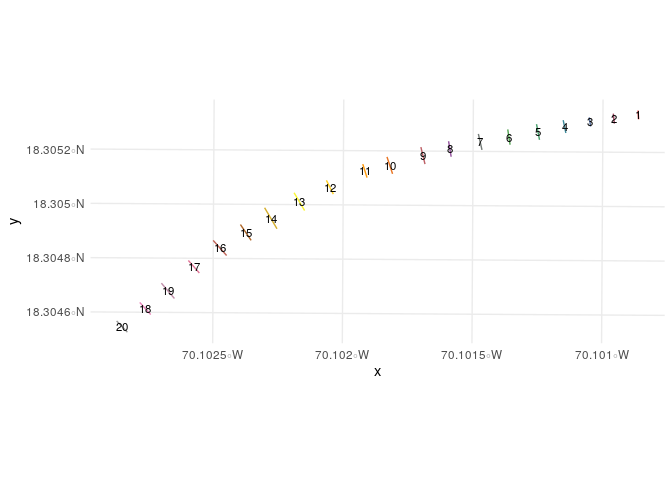
\includegraphics[height=3.12500in]{carolain-2.png}
\caption{mapa de perfil de playa transectos\label{transectos-playa}}
\end{figure}

\begin{Shaded}
\begin{Highlighting}[]
\NormalTok{Profile data}
\NormalTok{profData_temp <-}\StringTok{ }\KeywordTok{profiles}\NormalTok{(}\DataTypeTok{transects =}\NormalTok{ transprof, }\DataTypeTok{height =}\NormalTok{ dsm,}
                          \DataTypeTok{pointsPerPixel=} \DecValTok{2}\NormalTok{, }\DataTypeTok{movingAvgK =} \DecValTok{3}\NormalTok{)}
\NormalTok{## rgeos version: 0.5-1, (SVN revision 614)}
\NormalTok{##  GEOS runtime version: 3.6.2-CAPI-1.10.2 }
\NormalTok{##  Linking to sp version: 1.3-1 }
\NormalTok{##  Polygon checking: TRUE}
\NormalTok{## }
\NormalTok{## Attaching package: 'scales'}
\NormalTok{## The following object is masked from 'package:purrr':}
\NormalTok{## }
\NormalTok{##     discard}
\NormalTok{## The following object is masked from 'package:readr':}
\NormalTok{## }
\NormalTok{##     col_factor}
\NormalTok{## }
\NormalTok{## Attaching package: 'zoo'}
\NormalTok{## The following objects are masked from 'package:base':}
\NormalTok{## }
\NormalTok{##     as.Date, as.Date.numeric}
\NormalTok{## udunits system database from /usr/share/xml/udunits}
\NormalTok{profData_temp}
\NormalTok{## $dimension}
\NormalTok{## # A tibble: 2,603 x 5}
\NormalTok{##    transect       dist        h      hma     distlm}
\NormalTok{##    <fct>           [m]      [m]      [m]        [m]}
\NormalTok{##  1 1        0.00000000 2.447498       NA         NA}
\NormalTok{##  2 1        0.04982810 2.447498 2.447221 0.04982810}
\NormalTok{##  3 1        0.09965621 2.446667 2.446944 0.09965621}
\NormalTok{##  4 1        0.14948432 2.446667 2.436445 0.14948432}
\NormalTok{##  5 1        0.19931242 2.416000 2.426222 0.19931242}
\NormalTok{##  6 1        0.24914053 2.416000 2.402000 0.24914053}
\NormalTok{##  7 1        0.29896863 2.374001 2.388000 0.29896863}
\NormalTok{##  8 1        0.34879674 2.374001 2.352666 0.34879674}
\NormalTok{##  9 1        0.39862484 2.309998 2.331332 0.39862484}
\NormalTok{## 10 1        0.44845295 2.309998 2.291665 0.44845295}
\NormalTok{## # … with 2,593 more rows}
\NormalTok{## }
\NormalTok{## $dimensionless}
\NormalTok{## # A tibble: 2,603 x 3}
\NormalTok{##    transect   distlm    hma}
\NormalTok{##    <fct>       <dbl>  <dbl>}
\NormalTok{##  1 1        NA       NA    }
\NormalTok{##  2 1         0        1    }
\NormalTok{##  3 1         0.00678  1.000}
\NormalTok{##  4 1         0.0136   0.996}
\NormalTok{##  5 1         0.0203   0.991}
\NormalTok{##  6 1         0.0271   0.982}
\NormalTok{##  7 1         0.0339   0.976}
\NormalTok{##  8 1         0.0407   0.961}
\NormalTok{##  9 1         0.0475   0.953}
\NormalTok{## 10 1         0.0542   0.936}
\NormalTok{## # … with 2,593 more rows}
\NormalTok{## }
\NormalTok{## $dimensionlessrawdistance}
\NormalTok{## # A tibble: 2,603 x 3}
\NormalTok{##    transect   dist    hma}
\NormalTok{##    <fct>     <dbl>  <dbl>}
\NormalTok{##  1 1        0      NA    }
\NormalTok{##  2 1        0.0143  1    }
\NormalTok{##  3 1        0.0286  1.000}
\NormalTok{##  4 1        0.0429  0.996}
\NormalTok{##  5 1        0.0571  0.991}
\NormalTok{##  6 1        0.0714  0.982}
\NormalTok{##  7 1        0.0857  0.976}
\NormalTok{##  8 1        0.1000  0.961}
\NormalTok{##  9 1        0.114   0.953}
\NormalTok{## 10 1        0.129   0.936}
\NormalTok{## # … with 2,593 more rows}
\NormalTok{## }
\NormalTok{## $concavityindex}
\NormalTok{## # A tibble: 20 x 2}
\NormalTok{##    transect       ci}
\NormalTok{##    <fct>       <dbl>}
\NormalTok{##  1 1         0.0136 }
\NormalTok{##  2 10        0.188  }
\NormalTok{##  3 11        0.371  }
\NormalTok{##  4 12        0.281  }
\NormalTok{##  5 13        0.149  }
\NormalTok{##  6 14        0.0692 }
\NormalTok{##  7 15        0.127  }
\NormalTok{##  8 16        0.0530 }
\NormalTok{##  9 17       -0.0744 }
\NormalTok{## 10 18       -0.0256 }
\NormalTok{## 11 19       -0.0809 }
\NormalTok{## 12 2         0.0173 }
\NormalTok{## 13 20        0.0441 }
\NormalTok{## 14 3         0.00273}
\NormalTok{## 15 4        -0.0295 }
\NormalTok{## 16 5        -0.0686 }
\NormalTok{## 17 6        -0.0428 }
\NormalTok{## 18 7         0.0276 }
\NormalTok{## 19 8         0.0960 }
\NormalTok{## 20 9         0.0880 }
\NormalTok{## }
\NormalTok{## $concavityindexrawdistance}
\NormalTok{## # A tibble: 20 x 2}
\NormalTok{##    transect      ci}
\NormalTok{##    <fct>      <dbl>}
\NormalTok{##  1 1        -0.454 }
\NormalTok{##  2 10        0.196 }
\NormalTok{##  3 11        0.381 }
\NormalTok{##  4 12        0.290 }
\NormalTok{##  5 13        0.0927}
\NormalTok{##  6 14       -0.0533}
\NormalTok{##  7 15       -0.267 }
\NormalTok{##  8 16       -0.335 }
\NormalTok{##  9 17       -0.364 }
\NormalTok{## 10 18       -0.605 }
\NormalTok{## 11 19       -0.693 }
\NormalTok{## 12 2        -0.261 }
\NormalTok{## 13 20       -0.699 }
\NormalTok{## 14 3        -0.412 }
\NormalTok{## 15 4        -0.420 }
\NormalTok{## 16 5        -0.228 }
\NormalTok{## 17 6        -0.218 }
\NormalTok{## 18 7        -0.141 }
\NormalTok{## 19 8        -0.0366}
\NormalTok{## 20 9        -0.0357}
\NormalTok{## }
\NormalTok{## $slope}
\NormalTok{## # A tibble: 20 x 10}
\NormalTok{##    transect       dh  ddistlm    slope slopeRad slopeDeg distrawd sloperawd}
\NormalTok{##    <fct>         [m]      [m]      [1]    [rad]      []      [m]       [1]}
\NormalTok{##  1 1        2.44722…  7.3495… -0.3077… -0.2985… -17.105… 3.487967 -0.29995…}
\NormalTok{##  2 10       0.69277…  7.1472… -0.0495… -0.0495…  -2.838… 7.220751 -0.04896…}
\NormalTok{##  3 11       0.79599…  5.5760… -0.1243… -0.1237…  -7.088… 5.675620 -0.12404…}
\NormalTok{##  4 12       0.50111…  6.1443… -0.0582… -0.0582…  -3.335… 6.244295 -0.05801…}
\NormalTok{##  5 13       1.18099…  8.9929… -0.0992… -0.0988…  -5.665… 8.384193 -0.09890…}
\NormalTok{##  6 14       1.47791… 11.4141… -0.1163… -0.1158…  -6.637… 9.903715 -0.11625…}
\NormalTok{##  7 15       1.63559… 12.7956… -0.1067… -0.1063…  -6.095… 7.740399 -0.10570…}
\NormalTok{##  8 16       2.06222… 13.9498… -0.1180… -0.1175…  -6.732… 8.195824 -0.11558…}
\NormalTok{##  9 17       2.19796…  9.3141… -0.2411… -0.2366… -13.556… 6.739649 -0.24007…}
\NormalTok{## 10 18       3.23785… 14.1406… -0.2272… -0.2234… -12.800… 6.566238 -0.22167…}
\NormalTok{## 11 19       2.58242… 16.7464… -0.1330… -0.1322…  -7.580… 8.001098 -0.12513…}
\NormalTok{## 12 2        1.98118…  5.6527… -0.3450… -0.3322… -19.034… 4.021715 -0.34471…}
\NormalTok{## 13 20       3.93166… 19.0466… -0.2038… -0.2010… -11.519… 6.080869 -0.19600…}
\NormalTok{## 14 3        1.71110…  6.4661… -0.2595… -0.2539… -14.552… 3.585818 -0.25854…}
\NormalTok{## 15 4        1.48999…  7.9341… -0.1942… -0.1918… -10.991… 5.237396 -0.19329…}
\NormalTok{## 16 5        1.24952…  7.6193… -0.1697… -0.1680…  -9.631… 6.446877 -0.16943…}
\NormalTok{## 17 6        1.03875…  7.3895… -0.1299… -0.1292…  -7.406… 6.261463 -0.12911…}
\NormalTok{## 18 7        0.93711…  7.8793… -0.1004… -0.1001…  -5.738… 6.625684 -0.09973…}
\NormalTok{## 19 8        0.78908…  7.7018… -0.0528… -0.0528…  -3.025… 6.356535 -0.05095…}
\NormalTok{## 20 9        0.76317…  8.1651… -0.0673… -0.0672…  -3.852… 7.082702 -0.06664…}
\NormalTok{## # … with 2 more variables: sloperawdRad [rad], sloperawdDeg []}

\NormalTok{Prepare data to accommodate }\DecValTok{48}\NormalTok{ profiles}
\NormalTok{profData <-}\StringTok{ }\KeywordTok{lapply}\NormalTok{(profData_temp, }\ControlFlowTok{function}\NormalTok{(x)}
\NormalTok{  x }\OperatorTok\StringTok{ }\KeywordTok{mutate}\NormalTok{(}
    \DataTypeTok{transect2 =} \KeywordTok{as.numeric}\NormalTok{(}\KeywordTok{as.character}\NormalTok{(transect)),}
    \DataTypeTok{group =} \KeywordTok{cut}\NormalTok{(transect2,}
                \DataTypeTok{breaks =} \KeywordTok{c}\NormalTok{(}\DecValTok{0}\NormalTok{, }\DecValTok{5}\NormalTok{, }\DecValTok{10}\NormalTok{, }\DecValTok{15}\NormalTok{, }\DecValTok{20}\NormalTok{),}
                \DataTypeTok{labels =} \KeywordTok{c}\NormalTok{(}\StringTok{'1-5'}\NormalTok{, }\StringTok{'6-10'}\NormalTok{, }\StringTok{'11-15'}\NormalTok{, }\StringTok{'16-20'}\NormalTok{)),}
  \DataTypeTok{transect =}\NormalTok{ forcats}\OperatorTok{::}\KeywordTok{fct_relevel}\NormalTok{(}
\NormalTok{    transect, }\ControlFlowTok{function}\NormalTok{(x)\{}\KeywordTok{as.character}\NormalTok{(}\KeywordTok{sort}\NormalTok{(}\KeywordTok{as.integer}\NormalTok{(x)))\})}
\NormalTok{  )}
\NormalTok{)}
\NormalTok{Profile plots}
\NormalTok{Dimensionsional profiles}
\NormalTok{Profiles match their actual digitized }\KeywordTok{extension}\NormalTok{ (raw distance)}
\NormalTok{xy scales different, scale non}\OperatorTok{-}\NormalTok{consistent across panels}
\CommentTok{#Raw distance}

\NormalTok{dmngrid <-}\StringTok{ }\KeywordTok{sapply}\NormalTok{(}\KeywordTok{as.character}\NormalTok{(}\KeywordTok{unique}\NormalTok{(profData}\OperatorTok{$}\NormalTok{dimension}\OperatorTok{$}\NormalTok{group)), }\ControlFlowTok{function}\NormalTok{(x) \{}
\NormalTok{  profData}\OperatorTok{$}\NormalTok{dimension }\OperatorTok\StringTok{ }\KeywordTok{filter}\NormalTok{(group}\OperatorTok{==}\NormalTok{x) }\OperatorTok\StringTok{ }\NormalTok{drop_units }\OperatorTok\StringTok{ }\KeywordTok{ggplot}\NormalTok{() }\OperatorTok{+}
\StringTok{    }\KeywordTok{aes}\NormalTok{(}\DataTypeTok{x =}\NormalTok{ distlm, }\DataTypeTok{y =}\NormalTok{ hma) }\OperatorTok{+}
\StringTok{    }\KeywordTok{geom_line}\NormalTok{(}\DataTypeTok{col =} \StringTok{'red'}\NormalTok{, }\DataTypeTok{lwd =} \DecValTok{1}\NormalTok{, }\DataTypeTok{na.rm =}\NormalTok{ T) }\OperatorTok{+}
\StringTok{    }\KeywordTok{scale_x_continuous}\NormalTok{(}\DataTypeTok{breaks =} \KeywordTok{pretty_breaks}\NormalTok{()) }\OperatorTok{+}
\StringTok{    }\KeywordTok{scale_y_continuous}\NormalTok{(}\DataTypeTok{breaks =} \KeywordTok{pretty_breaks}\NormalTok{()) }\OperatorTok{+}
\StringTok{    }\KeywordTok{expand_limits}\NormalTok{(}\DataTypeTok{y =} \OperatorTok{-}\FloatTok{0.05}\NormalTok{) }\OperatorTok{+}
\StringTok{    }\KeywordTok{ylab}\NormalTok{(}\StringTok{'Height, moving average (m)'}\NormalTok{) }\OperatorTok{+}\StringTok{ }\KeywordTok{xlab}\NormalTok{(}\StringTok{'Distance, landward origin (m)'}\NormalTok{) }\OperatorTok{+}
\StringTok{    }\KeywordTok{geom_text}\NormalTok{(}
      \DataTypeTok{data =}\NormalTok{ profData}\OperatorTok{$}\NormalTok{slope }\OperatorTok\StringTok{ }\KeywordTok{filter}\NormalTok{(group}\OperatorTok{==}\NormalTok{x) }\OperatorTok\StringTok{ }\NormalTok{drop_units,}
      \KeywordTok{aes}\NormalTok{(}\DataTypeTok{x =} \DecValTok{0}\NormalTok{, }\DataTypeTok{y =} \DecValTok{0}\NormalTok{, }\DataTypeTok{label =} \KeywordTok{paste0}\NormalTok{(}\StringTok{'m='}\NormalTok{, }\KeywordTok{round}\NormalTok{(slopeDeg,}\DecValTok{2}\NormalTok{),}\StringTok{' '}\NormalTok{ )),}
      \DataTypeTok{size =} \DecValTok{3}\NormalTok{,}
      \DataTypeTok{hjust =} \DecValTok{0}\NormalTok{,}
      \DataTypeTok{parse =}\NormalTok{ F}
\NormalTok{    ) }\OperatorTok{+}
\StringTok{    }\KeywordTok{facet_wrap}\NormalTok{(}\OperatorTok{~}\NormalTok{transect, }\DataTypeTok{nrow =} \DecValTok{2}\NormalTok{, }\DataTypeTok{scales =} \StringTok{'free'}\NormalTok{) }\OperatorTok{+}
\StringTok{    }\KeywordTok{theme_bw}\NormalTok{() }\OperatorTok{+}\StringTok{ }
\StringTok{    }\KeywordTok{theme}\NormalTok{(}\DataTypeTok{text =} \KeywordTok{element_text}\NormalTok{(}\DataTypeTok{size =} \DecValTok{8}\NormalTok{))}
\NormalTok{\}, }\DataTypeTok{simplify =}\NormalTok{ F, }\DataTypeTok{USE.NAMES =}\NormalTok{ T)}

\KeywordTok{invisible}\NormalTok{(}\KeywordTok{sapply}\NormalTok{(}
  \KeywordTok{names}\NormalTok{(dmngrid),}
  \ControlFlowTok{function}\NormalTok{(x) \{}
    \KeywordTok{print}\NormalTok{(dmngrid[[x]])}
\NormalTok{  \}}
\NormalTok{))}

\KeywordTok{invisible}\NormalTok{(}\KeywordTok{sapply}\NormalTok{(}
  \KeywordTok{names}\NormalTok{(dmngrid),}
  \ControlFlowTok{function}\NormalTok{(x) \{}
\NormalTok{    p <-}\StringTok{ }\NormalTok{dmngrid[[x]] }\OperatorTok{+}
\StringTok{      }\KeywordTok{stat_smooth}\NormalTok{(}
        \KeywordTok{aes}\NormalTok{(}\DataTypeTok{x =}\NormalTok{ distlm, }\DataTypeTok{y =}\NormalTok{ hma), }\DataTypeTok{geom =} \StringTok{'line'}\NormalTok{, }\DataTypeTok{color =} \StringTok{'black'}\NormalTok{,}
        \DataTypeTok{alpha =} \FloatTok{0.5}\NormalTok{, }\DataTypeTok{formula =}\NormalTok{ y}\OperatorTok{~}\NormalTok{x, }\DataTypeTok{method =} \StringTok{'lm'}\NormalTok{, }\DataTypeTok{na.rm =}\NormalTok{ T) }\OperatorTok{+}
\StringTok{      }\KeywordTok{scale_x_continuous}\NormalTok{(}\DataTypeTok{limits =} \KeywordTok{c}\NormalTok{(}\DecValTok{0}\NormalTok{,}\DecValTok{13}\NormalTok{)) }\OperatorTok{+}
\StringTok{      }\KeywordTok{scale_y_continuous}\NormalTok{(}\DataTypeTok{limits =} \KeywordTok{c}\NormalTok{(}\DecValTok{0}\NormalTok{,}\FloatTok{2.5}\NormalTok{)) }\OperatorTok{+}\StringTok{      }
\StringTok{      }\KeywordTok{facet_wrap}\NormalTok{(}\OperatorTok{~}\NormalTok{transect, }\DataTypeTok{nrow =} \DecValTok{5}\NormalTok{) }\OperatorTok{+}\StringTok{ }\KeywordTok{coord_equal}\NormalTok{()}
    \KeywordTok{print}\NormalTok{(p)}
\NormalTok{  \}}
\NormalTok{))}
\end{Highlighting}
\end{Shaded}

\section{Referencias}\label{referencias}

\begin{center}\rule{0.5\linewidth}{\linethickness}\end{center}

\hypertarget{refs}{}
\hypertarget{ref-jose_ramon_martinez_batlle_2020_3937481}{}
Batlle, J. R. M. (2020). Geofis/rcoastsat: RCoastSat (Version
v0.0.0.9000). \url{https://doi.org/10.5281/zenodo.3937481}

\hypertarget{ref-carranza2010causas}{}
Carranza-Edwards, A. (2010). Causas y consecuencias de la erosión de
playas. \emph{Impacto Del Cambio Climático Sobre La Zona Costera:
México, Instituto de Ecología, AC (INECOL), Texas Sea Grant Program,
Instituto Nacional de Ecología (INE-SEMARNAT)}, 36--50.

\hypertarget{ref-codignotto1997geomorfologia}{}
Codignotto, J. (1997). \emph{Geomorfología y dinámica costera}.

\hypertarget{ref-jackson2005glossary}{}
Jackson, J. A. (2005). Glossary of geology. \emph{Glossary of Geology,
by JA Jackson. 2005 Approx. 900 P. 5th Revised and Enlarged Ed. ISBN
3-540-27951-2. Berlin: Springer, 2005.}, 5th.

\hypertarget{ref-mollat2004mapa}{}
Mollat, H., Wagner, B. M., Cepek, P., \& Weiss, W. (2004). \emph{Mapa
Geológico de la República Dominicana 1:250.000. Texto Explicativo}.
Stuttgart: E. Schweizerbart'sche Verlagsbuchhandiung.

\hypertarget{ref-ortiz1992retroceso}{}
Ortiz Pérez, M. A. (1992). Retroceso reciente de la línea de costa del
frente deltaico del río san pedro, campeche-tabasco.
\emph{Investigaciones Geográficas}, (25), 7--23.

\hypertarget{ref-pedraza1996geomorfologia}{}
Pedraza Gilsanz, J. de. (1996). \emph{Geomorfología: Principios, métodos
y aplicaciones}.

\hypertarget{ref-kilian_vos_2019_3560436}{}
Vos, K., Splinter, K., Leaman, C., \& ianlturner. (2019). Kvos/coastsat:
CoastSat v1.0.1 (Version v1.0.1).
\url{https://doi.org/10.5281/zenodo.3560436}




\newpage
\singlespacing 
\end{document}
